% This template was written by John Davies <john.davies@glasgow.ac.uk> 2017-02-06
% It matches the university specification at the time of writing
%   for the widths of the page margins and one-and-a-half line spacing
% You may want to include more packages, particularly for heavy mathematics
% Please let me know if you find any errors or wish to suggest improvements

\documentclass[12pt,titlepage,oneside]{book}
\usepackage[T1]{fontenc} % modern encoding
% Comment out the next three lines of LaTeX if you wish to use Computer Modern fonts
%   (this is the default for LaTeX)
% Make sure that your TeX installation can produce good pdf with these fonts.
% The following three lines are a good alternative if you don't use much mathematics
\usepackage{mathptmx}  % uses Times for text and mathematics
\usepackage[scaled]{helvet} %  helvetica for sanserif, scaled 95% by default
\usepackage{courier}  % courier for typewriter font, pretty ugly but available
% otherwise the stix package offers more options and symbols
% \usepackage{stix}  % uses Times for text and a range of fonts for mathematics
% End of choices for fonts
\usepackage{graphicx}  % standard package for importing graphics files
\usepackage{cite}  % improves format of numerical citations, such as [1-3]
\usepackage[top=1.8cm, bottom=1.8cm,left=4.0cm,right=1.5cm]{geometry}
% These margins are the university guidelines
\usepackage[onehalfspacing]{setspace}  % gives one-and-a-half line spacing
% doublespacing is another option and can be changed in the text
\usepackage{dcolumn}   % needed for some tables
\usepackage{bm}        % for math
\usepackage{amssymb}   % for math
\usepackage{amsmath}
\usepackage{color}
\usepackage{acronym}
\usepackage{algcompatible}
\usepackage{newfloat}
\usepackage{cancel}
\usepackage{subcaption}
\graphicspath{{./figures/}}
\usepackage{hyperref}
\usepackage{sidecap}


\sidecaptionvpos{figure}{c}

\DeclareFloatingEnvironment[
    fileext=loa,
    listname=List of Algorithms,
    name=ALGORITHM,
    placement=tbhp,
]{algorithm}

\newcommand{\joe}[1]{\textbf{\textcolor{red}{JOE: #1}}}

\begin{document}
\begin{titlepage}
\centering
\vspace*{3cm}  % Need the * or the space is swallowed at the top of the page
\bfseries\Large
Data Analysis Techniques for Continuous Gravitational Wave Searches\\
\vspace{3cm}
\normalfont\large
Joseph Bayley\\
\vspace{2cm}
Submitted in fulfilment of the requirements for the\\
Degree of Doctor of Philosophy\\
\vspace{2cm}
School of Physics and Astronomy\\
College of Science and Engineering\\
University of Glasgow\\
\vspace{1cm}
\includegraphics[scale=0.125]{GlaLogo.pdf}
\\
\vspace{1cm}
% Insert month and year of date deposited with library for final version
February 2017
\end{titlepage}
\frontmatter  % Turn off chapter numbering, use roman page numbers
\chapter{Abstract}

The field of gravitational wave astronomy is still in its early stages, with
detections of compact binary coalescences numbering $\sim
60$~\chris{techncially we haven't claimed that ythe O3 events are indeed
detections. We still only have 11 from O1 and O2 plus the recent BNS and
GW190412. All other events are "candidates".}. Another possible source of
gravitational waves is rapidly rotating neutron stars which have some asymmetry
around their rotation axis~\chris{ambiguous - are they possible source AND they
have asymmetry or are they possible sources BECAUSE they have asymmetry?}.
These are predicted to emit long duration quasi-sinusoidal signals known as
continuous gravitational waves.

% SOAP chapter
All-sky and wide parameter space searches for continuous gravitational waves
are generally template-matching schemes which test a bank of signal waveforms
against data from a gravitational wave detector.  Such searches can offer
optimal~\chris{I'd be careful here. There is no optimality at play. Really,
it's a case of having an algorithm and then tuning its own sensitivity at a
fixed computational cost. Your algorithm is basically as sensitive as others
but uses a tiny fraction of the cost so you can't say that any of the
approaches are "optimal".} sensitivity for a given computing cost and signal
model, but are highly-tuned to specific signal types and are computationally
expensive, even for semi-coherent~\chris{try to keep techncial jargon out of
the abstract} searches. We have developed a search method based on the Viterbi
algorithm which is model-agnostic and has a computational cost several orders
of magnitude lower than template methods,~\chris{and} with a modest reduction
in sensitivity~\chris{is this true? I thought we were in the mix compared to
all the semi-coherent approaches.}. In particular, this method can search for
signals which have an unknown frequency evolution. We test the algorithm on
three simulated and real data sets: gapless Gaussian noise, Gaussian noise with
gaps and real data from the final run of initial LIGO (S6). We show that at
95\% efficiency, with a 1\% false alarm rate, the algorithm has a depth
sensitivity~\chris{depth is a bit technical unless defined. It's relatively
simple to define so you might think about saying "depth sensitivity
$S_{h}(f)/h_0$" of $\ldots$. Careful to then also define the variables. It
might be a bit messy.} of $\sim 33$, $10$ and $13$\,Hz$^{-1/2}$ with
corresponding ~\chris{it's important to state that this is the optimal coherent
SNR and not the SNR of the viterbi statistic.} SNRs~\chris{careful with
undefined acronymns} of $\sim 60$, $72$ and $74$ in these datasets. We discuss
the use of this algorithm for detecting a wide range of quasi-monochromatic
gravitational wave signals and instrumental lines~\chris{jargon?}, and
demonstrate that it can also highlight~\chris{highlight is vague. What does
that mean?} shorter duration signals such as compact binary coalescences.


% Machine learning chapter
Many continuous gravitational wave searches are affected by instrumental lines
as the long duration narrowband nature of a line can appear to be very similar
to a real continuous~\chris{gravitational?} wave signal.  This has led
to~\chris{the development of} techniques to try and limit the effect of
instrumental lines, which mostly involve developing a statistic to penalise
signals that appear in only a single detector.  We have developed a method
using convolutional neural networks to reduce the impact of instrumental
artefacts on the SOAP~\chris{SOAP hasn't been defined.} search.  This has the
ability to identify features in each detectors spectrograms such that a
frequency band can be classified into a signal or noise class.  Using this
method we achieve a similar sensitivity to the SOAP search alone~\chris{make
this clearer to the reader. I know what you mean but it sounds like you've made
a change that has no effect}, however, this allows SOAP to be a fully
automated~\chris{the importance of automation is only important if the reader
knows about the manual line identification.} search which will return
candidates to be followed up.~\chris{this paragrpah can be made a lot clearer.}


% Parameter est chapter 
Once a continuous gravitational wave is detected, we would want to extract some
parameters associated with the source to help understand more about its
structure and evolution.  We describe a Bayesian method which extracts the sky
location, frequency and frequency derivative of a source associated with the
frequency evolution returned by the SOAP algorithm.  This has the aim of
limiting the size of the parameter space for a more sensitive fully coherent
follow up search.  We demonstrate a model which currently does not provide
valid estimates of the source parameters, however, with further investigation
we aim to develop this into a reliable analysis.~\chris{You maybe don't need to
be as bluntly negative and honest as you are here. I would advise slightly
expanding the description but also say that we present results and describe the
features and shortcomings of our approach. Or something like that. While we are
talimng about the PE, I would expect the results to be more presentable if you
take the 50\% confindence interval as opposed to the 95\%. Have you been bale
to do this yet?}

% Lines chapter
As mentioned above, we limit the effect of instrumental lines on the SOAP
search using machine learning, however we can also identify and mitigate these
lines separately before a search is run.  We demonstrate how we can use SOAP in
a simple configuration to identify instrumental lines.  We compare this method
to existing line identification tools used in the \gls{LIGO} collaboration, and
find that SOAP identifies many of the same lines as these methods as well as
some which do not appear on their line lists.~\chris{You could expand this a
bit but maybe more importtantly, since this is an abstract, you should make
some quantitative statements about the numbers/fractions of common lines found
as well as the numbers of new lines SOAP finds.}








\tableofcontents
\listoftables
\listoffigures
\include{acknowledgements}
\include{declaration}

\acrodef{GW}[GW]{gravitational-wave}
\acrodef{GR}[GR]{general relativity}
\acrodef{GRB}[GRB]{gamma ray burst}
\acrodef{CW}[CW]{continuous wave}
\acrodef{CBC}[CBC]{compact binary coalescence}
\acrodef{BBH}[BBH]{binary black hole}
\acrodef{BNS}[BNS]{binary neutron star}
\acrodef{NSBH}[NSBH]{neutron star black hole}
\acrodef{EMRI}[EMRI]{extreme mass ratio inspiral}
\acrodef{NS}[NS]{neutron star}
\acrodef{EOS}[EOS]{equation of state}
\acrodef{EM}[EM]{electromagnetic}
\acrodef{SNR}[SNR]{signal-to-noise-ratio}
\acrodef{LIGO}[LIGO]{Laser Interferometer Gravitational-wave Observatory}
\acrodef{SFT}[SFT]{short Fourier transform}
\acrodef{FFT}[FFT]{fast Fourier transform}
\acrodef{UCD}[UCD]{up, centre or down}
\acrodef{MDC}[MDC]{mock data challenge}
\acrodef{PSD}[PSD]{power spectral density}
\acrodef{ROC}[ROC]{receiver operating characteristic}
\acrodef{RMS}[RMS]{root median square}
\acrodef{MCMC}[MCMC]{Markov-Chain Monte Carlo}
\acrodef{SOAP}[SOAP]{snakes on a plane}
\acrodef{CNN}[CNN]{convolutional neural networks}

\mainmatter % Turn on chapter numbering, reset page numbers, use arabic
\chapter{Introduction}
%%%%%


Gravitational waves were first predicted by Einstein in 1915, as a consequence of his theory of \ac{GR} \cite{}. He then later theorised the gravitational waves in \cite{}.
The first observational evidence that \ac{GW} exist came from observations of the Hulse-Taylor binary \cite{}. 
This observation showed the binary pulsar system was in-spiraling and therefore losing energy.
This loss in energy matched the \ac{GR} prediction which assumed the energy was lost to \ac{GW}.
The in 2015 the first direct detection of gravitational waves was made by the \ac{LIGO} detectors in the US \cite{}.
This has then been followed my many more detection's involving \ac{LIGO} and Virgo \cite{}.

The field of gravitational wave astronomy is relatively new, it has the potential to offer a lot of new information on the behaviour and origins of the universe and the objects within. 
Up until their discovery in 2015 \cite{}, the only way to view the universe was through the electromagnetic spectrum or neutrinos. 
Gravitational waves offer a method to directly observe compact objects such as black holes and neutron stars. 
\ac{EM} radiation from any object is obscured by dust clouds and many other objects within the universe.
Due to gravity being a much weaker force, \acp{GW} do no react with these objects or dust, therefore, objects can be viewed without any obstruction. 

In this chapter I will introduce gravitational wave, their sources and how they are detected. 


%%%%%%%%%%%
%%%%%%%%%
\section{Gravitational waves}
%%%%%%%%%%%
%%%%%%%%%

In general relativity, gravity is caused by distortions in space-time, these distortions are cause by mass or energy. 
The larger the mass the more the space-time is distorted.
Gravitational waves are ripples in this space-time which propagate at the speed of light. 
\ac{GW} are a solution to the Einstein field equations,
\begin{equation}
    R_{\mu \nu} - \frac{1}{2}R g_{\mu \nu} = \frac{8 \pi G}{c^4}T_{\mu \nu}.
\end{equation}
where $R_{\mu \nu}$ is the Reimann tensor which describes the .............., $R$ is the Ricci scalar which is the trace of the Reimann tensor, $T_{\mu \nu}$ is the stress-energy tensor which desscribes the distribution of mass and energy in the universe and $g_\mu \nu$ us the metric tensor which describes the geometry of space-time.
I will not go into any detail on Einsteins field equations as they are a complicated set of equations.
However, I will mention that in a linearised theory, when pertubations to the metric tensor are assumed to be small, Einstein's field equations can be solved such that the solution is a plane wave. 
These pertubations to the metric tensor $g_{\mu \nu}$ are defined as,
\begin{equation}
    g_{\mu \nu} = \eta_{\mu \nu} + h_{\mu \nu},
\end{equation}
where $ \eta_{\mu \nu}$ is the metric for flat space-time and $h_{\mu \nu}$ is some small perturbation. 
The metric describes the geometry of space-time and is in general expected to be a flat space-time, i.e. $\eta_{\mu \nu} = \rm{diag}(-1,1,1,1)$.
The derivation of \ac{GW} has been summarised many times before, e.g. \cite{}, therefore, I will not repeat this here.
In empty space where $T_{\mu \nu} = 0$, the Einstein field equations give, 
\begin{equation}
    \Box h_{\mu \nu} = 0,
\end{equation}
which is a wave equation. 
This then has the solutions,
\begin{equation}
    h_{\plus} = \
    h_{\cross}
\end{equation}
Gives two polarisarions........
\joe{bits missing here}
\begin{figure}[h]
    \centering
    \includegraphics{}
    \caption{Shows how the polarisations affect free test masses}
    \label{gw:polarisations}
\end{figure}

In the post Newtonian expansion, the pertubation can be expressed as the second derivative of the quadrupole moment,
\begin{equation}
    h_{ij} = \frac{2G}{c^4}\frac{1}{r} \left [ \frac{d^2}{dt^2} Q_{ij} \right],
\end{equation}
where $G$ is the gravitational constant, $r$ is the distance to the source and $Q$ is the mass quadrupole moment defined as,
\begin{equation}
    Q_{ij} = \int \rho(x) \left(x_i x_j - \frac{1}{2}\delta_{ij} \right)dx^3,
\end{equation}
where $\rho$ is the mass density, and $x_i$ and $x_j$ are the coordinates.
This ultimately describes the non-spherical mass distribution within an objects. 
A quadrupole moment only exists when the mass distribution is not spherically symmetric, this is necessary for a \ac{GW} to be emitted.
This also shows how it is the acceleration of masses which is needed to produce gravitational waves.


\begin{itemize}
    \item Quadrupoles emit GW, masses which are not spherically symmetric around a rotation axis
    \item Quadrupole moments
    \item gravitational wave amplitude is proportinal to 2nd derivative of the quadrupole moment
    \item TT gauge
    \item polarisations, tidal forces, ring of masses plot
    \item need heavy objects to make them detectable 
\end{itemize}


%%%%%%%%%%%%%%
%%%%%%%%%%%%%
\section{\label{sources}Sources and signals}
%%%%%%%%%%%%%%%
%%%%%%%%%%%%%%%

There are many potential sources for \ac{GW}. The expected sources can be split into 3 general categories based on their signal type: Transient, Stochastic and \acp{CW}.
These categories are chosen based on the length of the signal and how well modelled the signal is.
Fig.~\ref{sources:signaltypes} shows an example of each of the signals as what category they are a part of.

\begin{figure}[h]
    \centering
    \includegraphics{}
    \caption{Each \ac{GW} signal type can be categorised based on its signal length and how well the signal is modelled.}
    \label{sources:signaltypes}
\end{figure}
In the sections that follow, I will give an overview of the potential sources of each of these signal categories and their waveforms.


%%%%%%%%%%%%%%%
\subsection{\label{sources:transient} Transient}
%%%%%%%%%%%%%%%

Transient sources of gravitational waves give short duration signal which is observable from milliseconds to tens of seconds depending on the source. 
Some of these sources will emit signals for a much longer time, however these are at a lower frequency and lower amplitude and not observable by current ground based detectors detectors.
Tranisent signals can be well modelled as in \acp{CBC} or unmodelled as in Burst signals.

\subsubsection{\label{sources:transient:cbc} Compact Binary Coalescence}

\acp{CBC} are well modelled signals which originate from the in-spiral and coalescence of compact objects. 
Compact objects include \acp{BBH}, \acp{BNS}, \acp{NSBH} and \acp{EMRI}.
\ac{BBH} and \ac{BNS} signals are currently the only sources which have been observed by the \ac{LIGO} and Virgo detectors \cite{}. 
The wave-forms of these sources which are observable by ground based detectors vary in length from less than a second to tens of seconds depending on the objects that make them.
In general higher mass systems such as \ac{BBH} inspiral faster and therefore have shorter signals.
However, they all have a similar form which is a `chirp' as shown in Fig.~\ref{sources:transient:cbc:wave}.

\begin{figure}[h]
    \centering
    \includegraphics{}
    \caption{CBC waveform}
    \label{sources:transient:cbc:wave}
\end{figure}


\ac{CBC} signals are generally split into three separate components: the inspiral, the merger and ring-down. 
The inspiral is when the objects are orbiting each other and as they lose energy to gravitational waves, the radius of the orbit decreases.
This continues until the objects begin to merge, which is when it reaches the merger phase.
After the objects have merged the remnant compact object 'rings down'. This means that the object still emits some gravitational waves as it settles into its final state.

In systems which have a neutron star, during the inspiral when the objects are close, the neutron star will begin to deform due to the strong gravity. 
This becomes useful as it will affect the generated waveform and can help determine the \ac{EOS} for the dense matter in a neutron star.
\ac{BNS} systems also offer a way do observe objects in multiple different channels, or what is known as multi-messenger astronomy. 
This is where the object can be viewed in the \ac{EM} spectrum as well as in gravitational waves.
This offers much in the field of astronomy as it can aid in the calculation of the Hubble constant. 


Black hole binaries have various formation channels, i.e. there are different way in which a compact binary system can form. 
These formation channels include: two high mass binary stars which collapse, two separate objects capture each other in their gravitational fields and begin to orbit etc..
However, exactly how common these are or if there are dominant ways in which they form is unknown. 
With many observations of \ac{CBC} it should be possible to discover which of these, if any, is dominant.

\begin{enumerate}
    \item BBH, BNS, BH-NS, EMRIs 
    \item can learn EOS from and neutron star interaction
    \item direct observation of black holes
    \item find their formation channels
    \item 
\end{enumerate}


%%%%%%%%%%%%%%
\subsubsection{\label{sources:transient:burst}Burst}
%%%%%%%%%%%%%%%%%

Burst sources are un-modelled and therefore have an unknown waveform.
This is because the sources could be unknown, or sources where the underlying physics of the system is not understood. 
Rather than generating wave-forms as in \ac{CBC} searches and using matched filtering, bursts usually look for short bursts in power which is coherent between detectors.

There are certain systems which could potentially emit a short duration burst like \ac{GW}.
These include core collapse supernovae \cite{}, \acp{GRB} \cite{}, .
Supernovae are when a massive star collapses and ejects its outer layers. 
If there is some asymmetry in the collapse then the system will emit some \ac{GW}.

\ac{GRB} are systems .........

In each of the example systems above, observing \ac{GW} gives a new insight into the processes happening inside hostile environments by giving an unobstructed view of them.

Ultimately burst searches are looking for signals which are unexpected, and are often flexible enough to look for any signal which appears consistently between detectors.

\begin{enumerate}
    \item High power which is consistent between detectors
    \item searches for uknown signal types
    \item these include: superova, GRB, etc
    \item can potentially probe what is happening is extreme environments
    \item but ultimately aim is to find something new
\end{enumerate}


%%%%%%%%%%%%%%%
\subsection{Stochastic}
%%%%%%%%%%%%%%%

\begin{enumerate}
    \item looks for unknown signal waveforms
    \item random fluctuations which are from many distant BBH overlapping
    \item inflation
\end{enumerate}

Stochastic gravitational waves have a few potential sources, however, their signal type is random background fluctuations. 
Some of the potential sources include a ensemble of distant \ac{BBH} signals which overlap, or from inflation which would be the cosmic microwave background equivalent. 

%%%%%%%%%%%%%%%%%%
\subsection{Continuous waves}
%%%%%%%%%%%%%%%%%%%%

\begin{itemize}
    \item rapidly roating neutron stars main source
    \item long duration continuously emitted
    \item can learn about EOS of dense neutron matter
    \item various emission possiblities
    \begin{itemize}
        \item "mountains" -> magnetic distortions -> crust distortions
        \item fundemental modes inside the neutron star -> fmode -> rmode
        \item precession
    \end{itemize}
    \item have been observed in EM
    \item 
\end{itemize}

Continuous \ac{GW} differ from the above categories as the signals are long duration, these waves are expected to last for much longer than observing runs of any detector. 
This gives an added benefit over other signals of being able to be located to great accuracy.

A primary source for continuous signals is expected to be rapidly rotation neutron stars (pulsars).
Neutron stars are thought to originate when the remnant of a massive star collapses, they are objects with incredibly high density and are highly magnetised.
Pulsars can be detected electromagnetically as they emit beamed radiation from the magnetic poles.
If the magnetic axis is not aligned with the rotation axis the radiation sweeps the detector at each rotation, this is detected as a pulsing signal which gave them their name \cite{lyne_graham-smith_2012}.
From electromagnetic observations, the rotation frequency of some pulsars can be observed to decrease with time, this is known as spin-down.
This spin-down means that the pulsar is losing energy somewhere, a fraction of this is thought to be due to gravitational waves. 

To emit gravitational waves the Pulsar has to have some asymmetry in its mass distribution around the rotation axis as spherically symmetric object do not emit gravitational waves.
There are a number of mechanisms which pulsars are thought to be able to emit gravitational waves by. The three leading mechanisms are: non-axisymmetric physical distortions in the star, vibrational modes and free precession \cite{Becker2009}.

%%%%%%
\subsubsection{Triaxial non-axisymmetry}
%%%%%%%%%

Triaxial non-axisymmetry is some deformation of the pulsar which is not symmetric around the rotation axis, this is often described as a `mountain' on its surface.

This assymmetry can be quantified by its ellipticity $\epsilon$,
\begin{equation}
\label{ellipticity}
\epsilon = \frac{I_{xx}-I_{yy}}{I_{zz}},
\end{equation}
where $I_{zz},I_{xx},I_{yy}$ are the principal moment of interia, where $I_{zz}$ is along the rotation axis. 
The ellipticity of a neutron star is expected to be $ \epsilon<10^{-5}$ \cite{Becker2009}. 
There are a number of theories which describe the origin of this axisymmetry.
If the pulsar is in a binary system and accreting material from its companion star, the material can be funnelled towards the magnetic poles by the magnetic field, thereby causing a hot spot.
This `hot spot' could cause a deformation on the surface of the star which is not axi-symmetric. 
The magnetic stresses from strong magnetic fields within the star, could potentially also cause non axi-symmetric deformations to the star.
Finally the spin down of the pulsar itself could cause stresses in the crust of the star until the point of breaking, its then after this break which could leave a distortion in the crust \cite{Becker2009}.

The gravitational waves are expected to be emitted at a frequency which is twice the rotation frequency of the neutron star.
 
 %%%%%%%%%%%%%%
 \subsubsection{Vibrational modes}
 %%%%%%%%%%%%%%%
There are a number of modes within a star such as fundamental (f-modes) and r-modes. 
Each of these waves are oscillation i the star similar to oscillations in the earth which are used for seismology.
The difference between the different modes are the restoring force bringing the perturbed state back to equilibrium.
the f-modes use gravity as the restoring force where the oscillations happen in the crust of the star.
The more promising of these for gravitational wave emission and detection is the r-mode \cite{Becker2009}.
These are oscillations in the superfluid neutron part of the star,
where the restoring force for the oscillations is the Coriolis effect from the rotation of the star.
These are thought to emit gravitational waves at $4/3$ the frequency of rotation \cite{Becker2009}.

%%%%%%%%%%%%%%%
\subsubsection{Free precession}
%%%%%%%%%%%%%%

Free precession is when the rotation axis is misaligned with the symmetry axis of the star so that the start `wobbles'. 
Free precession is expected to produce gravitational waves at a frequency the same as the rotation frequency and twice the rotation frequency \cite{Becker2009}. 


\subsection{Exotic sources}

\begin{enumerate}
    \item other unknown sources consistent between detectors
\end{enumerate}

%%%%%%%%%%%%%%%
%%%%%%%%%%%%%%
%%%%%%%%%%%%%%%
\section{\label{intro:detector}Detectors}
%%%%%%%%%%%%%%%%
%%%%%%%%%%%%%%
%%%%%%%%%%%%%%

The theory mentioned above and the indirect detection of gravitational waves from the Hulse-Taylor binary pulsar system left little doubt as to whether \ac{GW} existed. 
The real challenge was to design an instrument which could directly detect gravitational waves.
There were a number of different methods for the design of the instrument which includes: resonant bar detectors, both ground based and space based interferometers, pulsar timing arrays and Cosmic microwave background detectors. 
Resonant bar detectors were initially designed and built by Joseph Weber \cite{}.
These are large cylinders of metal which should resonate as a gravitational wave passes by. 
These detectors did not make a direct detection therefore, the majority of these are no longer operational excluding some alternate designs such as \joe{put the spherical one etc}\cite{}.
Pulsar timing arrays aimed to use the accurate timing of pulsars to measure distortions in space time as a gravitational wave passed between the detector and the pulsar. 
Whilst a detection has not been made with this method, these methods are still in use.
Cosmic microwave background detectors aimed to look for evidence of gravitational waves in the polarisations of the CMB. 
Despite the announcement of a detection in ..., these are yet to find any evidence.
The most commonly known design of a \ac{GW} detector is the ground based interferometer, these made the first detection of \ac{GW} in 2015 \cite{}.
These are the focus of this section as the analysis that will follow uses data from the \ac{LIGO} detectors in the US.

%%%%%%%%
%%%%%%%%%
\subsection{Laser Interferometers}
%%%%%%%%%%
%%%%%%%%%

Laser interferometers use the inteference of light to measure a length with high precision.
A simple design is shown in Fig.~\ref{}. 
Here it shows how the laser is split into two, each of these beams is reflected from a mirror and then it returns to the beam splitter where the two beams are combined.
At the output, there is an inteference pattern between the two beams.
If the length of one of the arms is changed then the inteference pattern will change as the phase of one beam changes with respect to the other.

This can be used in gravitational wave detection as the mirrors at the end of each arm of the interfereometer can be treated as `free' test masses.
This is what is shown in Fig.~\ref{detectors:interfereometer}, where a gravitational wave passing the masses will stretch and squeeze them, essentially changing the relative lengths of the two arms.
The intensity of the inteference pattern at a given point is then proportional to the gravitational wave itself.

\begin{figure}
    \centering
    \includegraphics{}
    \caption{This figure shows a basic interferometer.}
    \label{detectors:interfereometer}
\end{figure}

The actual gravitational wave detectors such as the \ac{LIGO} \cite{} and Virgo \cite{} detectors are much more complicated.
They use many techniques to reduce the noise from earth based sources and to increase the sensitivity to \ac{GW} signals.


%%%%%%%%%%%
%%%%%%%%%%
\subsubsection{Detector response}
%%%%%%%%%%
%%%%%%%%%

An important factor to know when using detector data to search for astrophysical signals is the detectors response.
This measures how sensitive the detector is to different locations on the sky.
An example of the antenna response for \ac{LIGO} is in Fig.~\ref{detectors:response}.
This is clear when thinking about how a gravitational wave affects the test masses. 
As the affect is transverse to the propagation of the wave, when the detector is face on to the source, there will be a maximum change in the arm lengths.

\begin{figure}
    \centering
    \includegraphics{}
    \caption{This figure shows the antenna response of one of the \ac{LIGO} detectors to sky position.}
    \label{detectors:response}
\end{figure}

%%%%%%%%%%%
%%%%%%%%%%
\subsubsection{Noise sources}
%%%%%%%%%%
%%%%%%%%%%
\begin{enumerate}
    \item Laser interferometers
    \item located US (LIGOs) Virgo
    \item detect the tidal deformations 
    \item mention instrumental lines for later section
    \item sensitivity curves
    \item future detectors
    \item antenna response
    \item 
\end{enumerate}

%%%%%%%%%%%%%
%%%%%%%%%%%%%%%
%%%%%%%%%%%%%%%%
\section{\label{intro:prob}Probability and Bayes Theorem}
%%%%%%%%%%%%%%%
%%%%%%%%%%%%%%%%
%%%%%%%%%%%%%%%%%

A key part in data analysis is understanding probability and statistics. 
This involves using basic probability along with the two general approaches to statistics: Bayesian and frequentist. 

%%%%%%%%%%%%%
%%%%%%%%%%%%%
\subsection{\label{intro:prob:basic}Basic probability}
%%%%%%%%%%%%%%
%%%%%%%%%%%%%%

We can define the probability of some event $A$ as $p(A)$ where probabilities follow $0 \leq p(A) \leq 1$ and some other event $B$ which has a probability $p(B)$ and follows $0 \leq p(B) \leq 1$.

\begin{description}
\item [Union]
A union is the probability of either and event $A$ happening or event $B$ happening, this is written as, $p(A \cup B)$.

\item [Intersection]
An intersection is then the probability of both and event $A$ and an event $B$ happens, this is written as $p(A \cap B)$.

\item [Independent and dependent Events]
If the events $A$ and $B$ are independent, i.e. the event $A$ does not affect the outcome of event $B$, then,
\begin{equation}
p(A \cap B) = p(A)p(B).
\end{equation}
However, if the event $A$ effects event $B$ then the joint probability of both events is,
\begin{equation}
\label{dependentevent}
p(A \cap B) = p(A)p(B \mid A) = p(B)p(A \mid B),
\end{equation}
where $p(B \mid A)$ means the probability of event $B$ happening given that event $A$ has happened.

\item [Conditional probability]
Conditional probability arises from situations where the outcome of one event will affect the outcome of future events.
The definition of this arises from the the dependent events defined above in Eq.~\ref{dependentevent},
\begin{equation}
p(A \mid B) = \frac{p(A \cap B)}{p(B)}.
\end{equation}

\item [Bayes Theorem]
Bayes theorem can then be defined using conditional probabilities. i.e we can use
\begin{equation}
p(A \mid B) = \frac{p(A \cap B)}{p(B)} \quad \rm{and} \quad p(B \mid A) = \frac{p(A \cap B)}{p(A)}
\end{equation}
such that then,
\begin{equation}
p(B)p(A \mid B) = p(A)p(B \mid A)
\end{equation}
and this is rearranged to Bayes theorem,
\begin{equation}
p(A \mid B) = \frac{p(A)p(B \mid A)}{p(B)}
\end{equation}

\end{description}

%%%%%%%%%%%%%%%%%
%%%%%%%%%%%%%%%%%%
\subsection{\label{intro:prob:bayes}Bayesian Inference}
%%%%%%%%%%%%%%%%%%%
%%%%%%%%%%%%%%%

We can take Bayes theorem from Sec.~\ref{intro:prob:basic} and apply it to a problem which involves infering some parameters from some model. Here we can relabel the events $A$ and $B$ with the data ${\bm d}$ and the parameters ${\bm \theta}$ of some model $I$.

\begin{equation}
p({\bm \theta} \mid {\bm d}, I) = \frac{p({\bm \theta}, I)p({\bm d} \mid {\bm \theta}, I)}{p(I)}
\end{equation}
where $p({\bm \theta} \mid {\bm d})$ is the posterior distribution, $p({\bm \theta})$ is the prior distribution,  $p({\bm d} \mid {\bm \theta})$ is the likelihood and $p({\bm d})$ is the evidence.

\begin{description}
\item [Posterior]
The posterior distribution describes the probability of getting certain values of parameters within a model given some data. 
\item [Prior]
The Prior is the element which can be left open to the users interpretation. This describes what you know about the model or the parameters of the model before you have seen any data. 
\item [Likelihood]
The likelihood contains information about how well the data matches the model with particular parameters. 
\item [Evidence]
The evidence is the probability of the data itself, i.e. it explains how likely this data is given and parameters within this model. 
\end{description}

\subsection{MCMC methods}

\subsection{Nested sampling}


% and the other chapters

\chapter{Continuous gravitational waves}


%%%%%%%%%%%%%%%%%%%%
%%%%%%%%%%%%%%%%%%%%
%%%%%%%%%%%%%%%%%%%
\section{\label{intro:search}Searching for Continuous gravitational waves}
%%%%%%%%%%%%%%%%%%%
%%%%%%%%%%%%%%%%%%%
%%%%%%%%%%%%%%%%%%

%%%%%%%
%%%%%%
\subsection{\label{intro:search:signals} Signals in data}
%%%%%%%
%%%%%%

The data recorded from a detector, $x(t)$, will include the signal model described in Eq.~\ref{sigmod} above, but it will be buried in the noise of the detector. 
If we assume the noise is Gaussian distributed and the noise and signal add linearly, then,  
\begin{equation}
\label{signalinnoise}
x(t) = n(t) + h(t; \mathcal{A},{\boldsymbol \lambda}) ,
\end{equation}
where $n(t)$ is the noise, $h(t)$ is the signal and $\mathcal{A}$ and ${\boldsymbol \lambda}$ refer to the amplitude and Doppler parameters respectively. 
The optimal signal to noise ratio (SNR) squared of this signal is defined as the scalar product of the signal with itself,
\begin{equation}
\rho^2(0) = ({\bf h} \mid {\bf h}) = \sum_X(h^X \mid h^X),
\end{equation}
where if there is more than one detector the SNR squared for each detector $X$ can be summed \citep{Prix2007}. 
The scalar product of two time series, $x(t)$ and $y(t)$, is defined by,

\begin{equation}
\label{intro:search:signals:scalarproduct}
(x \mid y) = 4 \Re \int_{0}^{\infty} \frac{\tilde{x}(f)\tilde{y}^{*}(f)}{S_n(f)}df,
\end{equation}
where $\tilde{x}(f)$ is the Fourier transform of $x(t)$, $\tilde{y}^{*}(f)$ is the complex conjugate of the Fourier transform of $y(t)$ and $S_n(f)$ is the single sided noise power spectral density \citep{Prix2007}.


\subsection{\label{intro:search:model}Continuous signal model}

The mode of a \ac{GW} signal from a pulsar is relatively simple, it is a sinusoid at a fixed frequency with a parameter which accounts for the loss of energy to gravitational waves and other mechanisms (spin down). 
Here the signal is modelled to originate from an isolated triaxial neutron star rotating around a principal axis. 
The parameters of each pulsar can be split into two sections: the Doppler components ($\alpha,\delta,f,\dot{f}$) and its amplitude components ($\psi,\phi_0, \iota, h_0, \theta$); this ignores any orbital parameters which would be present if the star was in a binary systems.
In the reference frame of the source, the gravitational wave can be written as,
\begin{equation}
h_{+}(t) = A_{+}\cos{(\Phi(t))} \quad \rm{and} \quad h_{\times}(t) = A_{\times}\cos{(\Phi(t))},
\end{equation}
where $h_{+}(t)$ and $h_{\times}(t)$ refer to the two polarisations and $\Phi(t) = \phi_0 + \phi(t)$ is the phase evolution of the source. $A_+$ and $A_{\times}$ are defined as,
\begin{equation}
A_+ = \frac{1}{2}h_0(1+\cos^2{\iota}), \quad A_{\times} = h_0 \cos{\iota},
\end{equation}
where $\iota$ is the inclination angle of the source and $h_0$ is the gravitational wave amplitude. The amplitude $h_0$ is defined as,
\begin{equation}
h_0 = \frac{16\pi^2 G}{c^4} \frac{\epsilon I_{zz} \nu^2}{d},
\end{equation}
where $c$ is the speed of light, $G$ is the gravitational constant, $\epsilon $ is the ellipticity defined in Eq.~\ref{ellipticity}, $\nu$ is the rotation frequency of the star and $d$ is its distance. 

To find the signal model in the detector frame one has to include the effects of the detector and its Doppler modulation as it moves through space. 
The Doppler modulation is included in the phase model such that now the phase follows, $\Phi(t) = \phi_0 + \phi(t, {\boldsymbol \lambda})$, where ${\boldsymbol \lambda}$ are the Doppler parameters. 
The amplitude of the signal is also modulated due to the orientation of the detectors relative to the source as the detector moves around the earth. These components are accounted for in the antenna patterns of the detector, defined in \citep{JKS1998} as,
\begin{equation}
\begin{split}
F_{+}(t) &= \sin{\zeta}[a(t)\cos{(2\psi)} + b(t)\sin{(2\psi)}], \\
F_{\times}(t) &= \sin{\zeta}[b(t) \cos{(2\psi)} - a(t)\sin{(2\psi)}],
\end{split}
\end{equation}
where $\zeta$ is the angle between the arms of the detectors, $\psi$ is the polarisation angle and $a(t)$ and $b(t)$ are defined in \citep{JKS1998}. 

The signal at the detector can then be written as a combination of the antenna patterns and the two polarisations of the gravitational wave,
\begin{equation}
h(t) = F_+(t)A_+\cos{[\phi_0 + \phi(t,{\boldsymbol \lambda})]} +F_{\times}(t)A_{\times}\sin{[\phi_0 + \phi(t,{\boldsymbol \lambda})]},
\end{equation}
The full signal model defined in \citep{JKS1998} actually includes all other parameters such as inclination angle, and has the form,
\begin{equation}
\label{sigmod}
%h(t) = F_{+}(t)[h_{1+}(t; h_0, \iota, \theta) + h_{2+}(t; h_0, \iota, \theta)] + F_{\times}(t)[h_{1\times}(t; h_0, \iota, \theta) + h_{2\times}(t; h_0, \iota, \theta)],
h(t) = F_{+}(t)[h_{1+}(t) + h_{2+}(t)] + F_{\times}(t)[h_{1\times}(t) + h_{2\times}(t)],
\end{equation}
where all parameters can be found in Eqs.~(21-22) of \citep{JKS1998}. 

%%%%%%
%%%%%%
\subsection{\label{intro:search:coherent}Fully-coherent searches}
%%%%%%
%%%%%%

Fully coherent searches are currently the most sensitive searches for continuous sources of gravitational waves. These searches are based on matched filtering which coherently correlate pre-generated waveforms with the data, this is used in \citep{Dupuis2005,Jaranowski1998,}.
In a simple form the matched filter filters the data $h$ with a template $w$ using the inner product defined in Eq.~\ref{intro:search:signals:scalarproduct}. 

Continuous wave signals need a large amount of integration time, $\mathcal{O}(\rm{years})$, for the signal to become clear within the data, therefore, given that the \ac{LIGO} detectors sample at 16 kHz, the amount of data to search over is large. 
Performing the coherent matched filter on this data can take a large amount of time, therefore, as the majority of sources which are searched for have a narrow bandwidth, many searches use techniques to reduce the amount of data. 
For example, in \citep{Dupuis2005} the data is heterodyned (mixed with some local oscillator), low passed filtered and then down-sampled. This reduced the amount of data to be searched over while not losing any source information. 

Whilst the fully coherent matched filter searches have methods to reduce the computational time for known sources, in all sky searches no parameters of the source are known, therefore, enough templates need to be made to sufficiently cover the large parameter space. 
This task quickly becomes impossible for coherent matched filtering for an entire observing run due to the amount of time needed. This problem led to the development of semi-coherent searches which will be introduced in the next section. 

%%%%%%
%%%%%%
\subsection{\label{intro:search:semicoherent}Semi-coherent searches}
%%%%%%
%%%%%%

Semi-coherent searches offered a solution to searching over large parameters spaces and large amounts of data. 
The data is split into smaller segments and the analysis is run separately on each of those segments, then each result is combined incoherently. 
This can greatly reduce the time taken for the analysis depending on the segment length, however, will always come with some loss in sensitivity. 

There are many different types of semi-coherent search which use various methods to incoherently combine the coherently analysed results. Many of these use 1800s (30 mins) \acp{SFT} as the input to their search as they can be calculated efficiently. 




\chapter{\label{viterbi}Viterbi Search}

To search for \ac{CW} signals, an adaptation of the Viterbi algorithm, which is well known in telecommunications, is used to search through spectrograms of \ac{LIGO} data. The basic idea of the search is simple, if we looked at a spectrogram frequency band as in Fig.~\ref{} we could find every possible track from a starting frequency bin to an end frequency bin (of which there are many). For each of these tracks the sum of the sprectrogram power along the track can be found such that for each track there is a single value, Fig.~\ref{} shows a histogram of these values. If there is a signal present in this band then it could be  assumed that the signal which gives the highest sum of spectrogram power is the track which is most likely to follow the signals frequency track.
Therefore, it can be assumed that if the frequency track with the highest sum of spectrogram power is found, then the corresponding track is most likely for follow a signal. 
Now as calculating all possible tracks is time consuming and the majority of tracks will not follow the signal track, it woudl be useful to have an algorithm which could find the maximum track more efficiently. This is where the Viterbi algorithm \cite{Viterbi} does this exact task. This is explained in the following sections.

\section{Viterbi algorithm}
%
% Into to viterbi
%
The Viterbi algorithm is an efficient method for determining the most probable set of states (a single `track' of steps on the time-frequency plane) in a Markov model dependent on data, where the model has a discrete number of states at each step. Rather than computing the probability of every possible track and selecting the most probable, the algorithm maximises this probability after every discrete step. As a result, a partial track which cannot ultimately be the most probable is rejected before the next step is calculated, and only a fraction of all possible tracks need to be computed to find the one that is most probable.

%
% Defining varibles and what data we use
%
In this work we apply the Viterbi algorithm to a \ac{GW} strain time-series to find the most probable track of a single variable-frequency signal in the noisy data.  We divide the time series into $N$ equal-length and contiguous segments ${\bm x}_j$,  defining the set $D \equiv \{{\bm x}_j\}$. The `states' in the model correspond to the frequencies a signal could have in each segment. A `track' is a list of such frequencies ${\bm \nu}\equiv \{\nu_j\}$, where  $\nu_j$ is the frequency in the segment ${\bm x_j}$.

%
% defining probabilities
%
Our objective is to calculate the most probable track given the data, i.e., the
track that maximises $p({\bm \nu}\mid D)$. Using Bayes theorem, this posterior probability can
be written as
%
\begin{equation}
\label{viterbi:bayes}
  p({\bm \nu} \mid D) = \frac{p({\bm \nu})p(D \mid {\bm \nu})}{p(D)},
\end{equation}
%
where $p({\bm \nu}) $ is the prior probability of the
track, $p(D \mid{\bm \nu})$ is the likelihood of the track (i.e., the
probability of the data given the track) and $p(D)$ is the model evidence (or
marginalised likelihood).

The Viterbi algorithm treats the track as the result of a Markovian process,
such that the current state depends only on the previous state. It is
therefore useful to split the track's prior into a set of transition
probabilities such that
%
\begin{align}
\label{viterbi:prior}
p({\bm \nu}) &= p(\nu_{N - 1}, \ldots, \nu_1, \nu_0)\nonumber \\
%&=  p(\omega_{N} \mid \omega_{N-1}, \ldots, \omega_1,\omega_0)p(\omega_{N-1} \mid \omega_{N-2}, \ldots, \omega_1,\omega_0) \ldots p(\omega_1 \mid \omega_0)p(\omega_0) \\
&= p(\nu_{N - 1} \mid \nu_{N-2})p(\nu_{N-2} \mid \nu_{N-3}) \dots p(\nu_1 \mid \nu_0)p(\nu_0) \nonumber \\
&= p(\nu_0)\prod_{j=1}^{N-1}p(\nu_{j} \mid \nu_{j-1}),
\end{align}
%
where $p(\nu_0)$ is the prior probability that the signal in the first time
step has a frequency $\nu_0$ and $p(\nu_{j} \mid \nu_{j-1})$ is the
prior `transition' probability for $\nu_j$ given the frequency at the last
step was $\nu_{j-1}$.

The noise in each of the segments can be treated as independent, so the
likelihood component in Eq.~\ref{viterbi:bayes} can be factorised as
%
\begin{equation}
\label{viterbi:likelihood}
p(D \mid {\bm \nu}) = \prod_{j=0}^{N-1}p({\bm x_j} \mid \nu_j),
\end{equation}
%
 where $p({\bm x_j} \mid \nu_j)$ is the likelihood of our
signal having a frequency $\nu_j$ in the $j$th segment.

Using Eqs.~\ref{viterbi:bayes},\ref{viterbi:prior} and
\ref{viterbi:likelihood}, the posterior probability is then
%
\begin{equation}
\label{viterbi:posterior}
    p({\bm \nu} | D) =
    \frac{p(\nu_0)p({\bm x_0} | \nu_0) \displaystyle\prod_{j=1}^{N-1}p(\nu_{j}
| \nu_{j-1})p({\bm x_j} | \nu_j)}{\displaystyle\sum_{S}
\left\{p(\nu_0)p({\bm x_0} | \nu_0)\displaystyle\prod_{j=1}^{N-1}p(\nu_{j} |
\nu_{j-1})p({\bm x_j} | \nu_j)\right\}} ,
\end{equation}
%
where in the denominator we must sum over all possible tracks
$S$~\cite{Slade2014}. We require the specific track, or set of frequencies, $\hat{\bm
\nu}$ that  maximises the posterior probability. Therefore, as the denominator in Eq.~\ref{viterbi:posterior} is a sum over all possible tracks, the track which maximises the posterior is the same track which
maximises the numerator  on the right-hand side of  Eq.~\ref{viterbi:posterior}, i.e.,
%
\begin{equation}
\label{viterbi:maxtrack}
  p(\hat{\bm \nu} | D) \propto \max_{\bm \nu}{\left[p(\nu_0)p({\bm x_0} |
\nu_0) \prod_{j=1}^{N-1}p(\nu_{j} |\nu_{j-1})p({\bm x_j} | \nu_j)\right]}.
\end{equation}
%
This track also maximises the log of the probability and can be written as,
%
\begin{equation}
\label{viterbi:maxtracklog}
\begin{split}
  \log p(\hat{\bm \nu} | D)  = \max_{{\bm \nu}}{\biggl\{ \log p(\nu_0) + \log p({\bm x_0} | \nu_0)  } \\
 \left. \sum_{j=1}^{N-1} \biggl[ \log p(\nu_{j} | \nu_{j-1}) + \log p({\bm x_j}
| \nu_j) \biggr] \right\} + \text{const}.
  \end{split}
\end{equation}
%
The Viterbi algorithm finds the most probable track $\hat{\bm \nu}$ by calculating the quantities in Eq,~\ref{viterbi:maxtracklog} for each frequency at each time step. In the following sections we explain how this is achieved in practice.

%%%%%%%%%%%%%%%%%%%%%%%%%%%%%%%%%%%%%%%%%%%%%%%%%%%%%%%%%%%%%%%%%%%%%%%%%
%%%%%%%%%%%%%%%%%%%%%%%%%%%%%%%%%%%%%%%%%%%%%%%%%%%%%%%%%%%%%%%%%%%%%%%%%
\section{\label{viterbi:transition}The transition matrix}
%%%%%%%%%%%%%%%%%%%%%%%%%%%%%%%%%%%%%%%%%%%%%%%%%%%%%%%%%%%%%%%%%%%%%%%%%
%
% define the transition matrix
%
An important concept when using the Viterbi algorithm is the`transition matrix' $T$, which is defined as the matrix that stores the prior log-probabilities $\log p(\nu_j \mid \nu_{j-1})$. These transition probabilities depend only on the size and direction of the transition, and in our case correspond to a jump in frequency when moving from the $(j-1)$th to the $j$th state. It is within the transition matrix that we impose some loose model constraints. For example it is usual in the time-frequency plane for frequencies to only have discrete values (frequency bins) and a track might only be allowed to move by one bin in each time step, restricting it to a \ac{UCD} transition or `jump' or equivalently setting the size of the first dimension of the transition matrix $n_1 = 3$. We can also impose that the transition probabilities are independent of the current track location in frequency, i.e. $p(\nu_j \mid \nu_{j-1})=p(\nu_{j+k} \mid \nu_{j+k-1})$. This leads to the transition matrix containing only three numbers, corresponding to the three prior log-probabilities that the track was in the corresponding \ac{UCD} frequency bin at the previous time step. These numbers are chosen to reflect the prior probability of a frequency deviation in the track and depend on the class of signals that one wishes to detect.
For the majority of examples that follow, a symmetric transition matrix is used, i.e. the probability of a transition up a frequency bin is equal to the probability of a transition down a frequency bin. This allows us to parameterise the one dimensional transition matrix with a single value, this value is the ratio of the probability of a transition to the same frequency bin, to either up or down a frequency bin. 

In later sections we will consider more complex situations in which the transition matrix describes the prior probability associated with sequences of even earlier transitions (`memory') and the case where there are multiple detectors. In these cases the number of dimensions of the transition matrix can grow substantially to account for the extra complexity of the problem.

%%%%%%%%%%%%%%%%%%%%%%%%%%%%%%%%%%%%%%%%%%%%%%%%%%%%%%%%%%%%%%%%%%%%%%%%%
%%%%%%%%%%%%%%%%%%%%%%%%%%%%%%%%%%%%%%%%%%%%%%%%%%%%%%%%%%%%%%%%%%%%%%%%%
\section{\label{viterbi:single}Single detector}
%%%%%%%%%%%%%%%%%%%%%%%%%%%%%%%%%%%%%%%%%%%%%%%%%%%%%%%%%%%%%%%%%%%%%%%%%
%
% single detector algorithm,
%
We will first consider the simple case of a single dataset $D$, generated by a single gravitational wave detector, and consider only a one-dimensional transition matrix. We will make use of discrete Fourier transforms so that frequencies, and hence the track frequencies, are also discrete. These frequencies will be indexed by $k$ and therefore $\nu_j \rightarrow \nu_{j,k}=k(j)\Delta f$ where $\Delta f=1/T$ is the frequency bin width for a segment of duration $T$.

 The Viterbi algorithm determines the most probable track on the time-frequency plane by calculating the value of Eq.~\ref{viterbi:maxtracklog} for every discrete Fourier frequency, incrementally in time. In other words, at each time segment it finds the most probable earlier track which ends at each particular frequency. On reaching the final segment it can look back to identify the most probable track connecting segment 1 to segment $N$.

There are two main components to Eq.~\ref{viterbi:maxtracklog}: the transition probabilities $p(\nu_j \mid \nu_{j-1})$ and the likelihoods $p({\bm x_j} \mid \nu_j)$. The transition probabilities are pre-calculated and stored in a transition matrix according to Sec.~\ref{viterbi:transition} above. To calculate the likelihood we follow the approach of~\cite{Bretthorst1988} which gives, under the assumption of a single sinusoidal signal in additive Gaussian noise in data segment ${\bm x_j}$, 

\joe{look at this is more detail, write more derivation, derive for log-odds as well as likelihood} 
%
\begin{equation}
\label{viterbi:single:likelihood}
p({\bm x_j} \mid \nu_{j,k}, \sigma_{j,k}, I) \propto
\exp\left[{C(\nu_{j,k})}\right].
\end{equation}
%
where
$C_{j,k}(\nu_{j,k})$ is the Schuster periodogram normalised to the noise variance at
frequency $\nu_{j,k}$ of segment $j$. This is equivalent to the log-likelihood, and is defined as
%
\begin{equation}
\label{viterbi:periodogram}
C(\nu_{j,k}) \equiv C_{j,k}=  \frac{1}{\sigma_{j,k}^2}\frac{1}{N_{\rm s}}\left|\sum_{r=0}^{N_{\rm
s}-1}x_{j,r} {\rm
e}^{i\nu_{j,k} t_r}\right|^2,
\end{equation}
%
where $N_{\rm s}$ is the number of data points in each segment and $t_{r}$ is the time corresponding to $x_{j,r}$, the $r$th sample in the $j$th data segment. $\sigma_{j,k}^2$ is the noise variance and is calculated as an estimate of the noise \ac{PSD} in the $k$th sample and the $j$th data segment. It is worth noting at this point that it is also possible to write this as a likelihood ratio, and therefore write out detection statistic as a log-odds ratio, however, we will discuss this in more depth in Sec.~\ref{viterbi:las}. The log-likelihoods of each segment can be calculated at discrete frequencies before running the algorithm by computing the power spectra for each segment from discrete Fourier transforms of the data. In the \ac{GW} field these standard data forms are known as \acp{SFT}.

The Viterbi algorithm records two quantities for each frequency and time bin: The first, $V_{j,k}$, contains the value defined by Eq.~\ref{viterbi:maxtracklog}, which is the log-probability of the most probable path ending in position $j,k$. The second, $A_{j,k}$, is the transition, or `jump', used to achieve the most probable path. The algorithm can be divided into three main sections: initialisation, iteration and identification. These three sections are described in pseudo-code in Alg.~\ref{viterbi:single:algorithm} and a simple demonstration of the algorithm at work is shown in Fig.~\ref{viterbi:plots}.
%
%
%   pseudo algorithm
%
\begin{algorithm}
\begin{algorithmic}[1]
\STATE{Input: ${C}$, $T$} \COMMENT{log-likelihood,transition matrix}
\STATE{Output: $\hat{\bm \nu}$, $V$, $A$} \COMMENT{most probable track, track probabilities, jumps}
\STATE
\STATE{ {\it Initialisation}}
\FOR{Frequency ($\nu_{0,k}$), $k=0 \rightarrow M-1$}
    \STATE{$V_{0,k} =  { C_{0k}} $ }
    \STATE{$A_{0,k} = 0$}
\ENDFOR
\STATE
\STATE{ {\it Iteration}}
\FOR{Segment, $j=0 \rightarrow N-1$}
    \FOR{Frequency ($\nu_{j,k}$), $k=0 \rightarrow M-1$}
        \STATE{$V_{j,k} = {\max\limits_{i }  ({ C_{j,k}} + T_i + V_{j-1,j+i})}$}
        \STATE{$A_{j,k} = {\argmax\limits_{ i }  ({ C_{j,k}} + T_i + V_{j-1,j+i})}$}
    \ENDFOR
\ENDFOR
\STATE
\STATE{ {\it Identification}}
\STATE{$\hat{\nu}_{N-1} = \argmax_k (V_{N-1,k})$}
\FOR{Segment, $j=N-1 \rightarrow 0$}
	\STATE{$\hat{\nu}_j = \hat{\nu}_{j+1} + A_{j,\nu_{k+1}}$}
\ENDFOR
%
\end{algorithmic}
\caption{The Viterbi algorithm in pseudo-code. $N$ is the number of segments, $M$ is the number of frequency bins in each segment. Here the maximisations over $i$ run between $\pm (n_1-1)/2$ where $n_1$ is the size of the transition matrix. The values from Eq.~\ref{viterbi:maxtracklog} are stored in $V$, and the jumps are stored in $A$. The most probable track is denoted by $\hat{\bm \nu}$.\label{viterbi:single:algorithm}}
\end{algorithm}
%
%
% example plot to work through
%
%
\begin{figure}
\centering
\begin{subfigure}[h]{0.8\columnwidth}
\includegraphics[width=0.8\columnwidth]{vit_data.pdf}
\caption{The input data}
\label{viterbi:plot:data}
\end{subfigure}

\begin{subfigure}[h]{0.8\columnwidth}
\includegraphics[width=0.8\columnwidth]{vit_prob.pdf}
\caption{The log-probabilities, jumps, and most probable path}
\label{viterbi:plot:likelihood}
\end{subfigure}

\caption{ Fig.~\ref{viterbi:plot:data} shows
the observed data, i.e the log-likelihood values $C_{j,k}$. Fig.~\ref{viterbi:plot:likelihood} shows the calculated
log-probabilities $V_{j,k}$. $A_{j,k}$ is shown in parentheses, where the \ac{UCD}
components correspond to $i= [-1,0,1]$ respectively. The red line shows the
path that gives the maximum probability. The transition matrix for the \ac{UCD} jumps is $[0,1,0]$ and corresponds to the un-normalised prior
log-probabilities of these jumps occurring.}
\label{viterbi:plots}
\end{figure}

\begin{description}
%
% Initialisation
%
\item[Initialisation] The two parts of Eq.~\ref{viterbi:maxtracklog},  $\log p(\nu_0)$ and $\log p({\bm x_0} \mid \nu_0)$, must be computed before the main recursive part of the algorithm can start. Therefore, the initialisation section (lines 5--8) in Alg.~\ref{viterbi:single:algorithm} calculates the first column in the lower panel of Fig.~\ref{viterbi:plots}. A priori, there is no preferred initial frequency, so we take the log-prior $\log p(\nu_{0,k})$ to be uniform over the complete frequency range. As a result, this is does not affect the maximisation for any jump, therefore, can be omitted from the calculation. We then use the pre-calculated log-likelihood values $C_{0,k}$ to fill the track probabilities $V_{0,k}$.  There is no previous position to jump from in this case, so the transition probabilities are irrelevant and $A_{0,k}$ are set to zero.
%
% Iteration
%
\item[Iteration] The main part of the calculation is the sum in Eq.~\ref{viterbi:maxtracklog}. Lines 11--16 in Alg.~\ref{viterbi:single:algorithm} calculate the most probable tracks that end at each frequency bin for each segment by using
    \begin{equation} \label{viterbi:single:vitsum}
    V_{j,k} = \max_{i}({C_{j,k} }+ T_{i} + V_{j-1,k+i}),
    \end{equation}
    where $i$ is the size and direction of the jump. For example, in Fig.~\ref{viterbi:plots} columns 1--4 are calculated in order using Eq.~\ref{viterbi:single:vitsum}, where it maximises over three possible previous positions in frequency. These positions are the frequency bins \ac{UCD} of the current position. The size and direction of the jump, $i$, which gives the maximum probability is then saved to $A_{j,k}$. These are shown in parentheses below the log-probabilities in Fig.~\ref{viterbi:plots} where \ac{UCD} correspond to values of $i = [-1,0,1]$ respectively.
%
% Identification
%
\item[Identification] The final stage of the algorithm identifies the most probable track. This is done by initially finding the highest log-probability values in the final time segment, $\max_k(V_{N-1,k})$ (line 19 in Alg.~\ref{viterbi:single:algorithm}). In the lower panel of Fig.~\ref{viterbi:plots} this is located at position $j,k = 4,1$ with $V_{4,1} = 22$. To find the track which corresponds to this, the values in $A_{jk}$ are followed backwards from this position (lines 20--21). For example, in Fig.~\ref{viterbi:plots} the final position is $j,k = 4,1$ and $A_{j,k} = \rm{Center} = 0$, this means that at the previous segment the most probable track was at position $j,k = 4-1,1+0 = 3,1$. At this time $A_{3,1} = R = 1$, therefore, the next track element is at $j,k = 3-1,1+1 = 2,2$. This then continues until $j=0$ whereupon these retraced positions constitute the most probable track, highlighted in red in Fig.~\ref{viterbi:plots}.
%
\end{description}

%
% mention the limitations - only returns max track.
%
The most probable track is the one traced backwards from the highest probability final segment frequency position. However, tracks can also be traced back from any of the end-frequency positions, returning the most probable track conditional on a given final position. Such tracks should not be confused with the being equal to the second, third, fourth, etc. most probable tracks. Information regarding the rankings and properties of all possible tracks (excluding the most probable and conditionally most probable tracks) is lost during the maximisation procedures computed at each stage in the algorithm --  a necessary consequence of the algorithm's speed and efficiency.

%%%%%%%%%%%%%%%%%%%%%%%%%%%%%%%%%%%%%%%%%%%%%%%%%%%%%%%%%%%%%%%%%%%%%%%%%
%%%%%%%%%%%%%%%%%%%%%%%%%%%%%%%%%%%%%%%%%%%%%%%%%%%%%%%%%%%%%%%%%%%%%%%%%
\section{\label{viterbi:multidet}Multiple detectors}
%%%%%%%%%%%%%%%%%%%%%%%%%%%%%%%%%%%%%%%%%%%%%%%%%%%%%%%%%%%%%%%%%%%%%%%%%
%
% introduce what multidetector means
%
If there are $Q$ detectors operating simultaneously we have $Q$ sets of data which can be combined appropriately to provide input to the Viterbi search described above. We must also modify the allowed transitions encoded within the transition matrix to take account of the extra prior constraints that are now available.

%
% Doppler shift at each detector
%
The received instantaneous frequency of a given astrophysical signal will be nearly the same for all ground-based \ac{GW} detectors, and our
algorithm should be sensitive to tracks that show this consistency in
frequency. However there \emph{will} be small differences between the frequencies measured at detectors that are not co-located, due to differential Doppler shifts caused by Earth rotation. As a result the signal could fall in different frequency bins at each detector.

\iffalse
To sufficient accuracy, the difference in frequency $\Delta f^{(1,2)}$ seen by two detectors ($1$ and $2$), is simply
%
\begin{equation}
\label{viterbi:multidet:doppler}
\Delta f^{(1,2)} = \frac{({{\bm v}^{(1)}} -{{\bm v}^{(2)}})\cdot{\bm \theta}}{c} f_0,
\end{equation}
%
where ${\bm v}_a$ is the velocity of detector $a$ in an inertial reference frame, $\bm \theta$ is a unit vector in the direction of the source and $f_0$ is the instantaneous signal frequency in the reference frame. The maximum difference would occur for two detectors on the equator separated by 180 degrees of longitude and for a source located in the equatorial plane, giving
%
\begin{equation}
\label{viterbi:multidet:doppler:diff}
\Delta f_{\rm max}  \approx 3.1\times 10^{-6} f_0.
\end{equation}
%
For a signal frequency of 200\,Hz the largest possible instantaneous difference in frequency between detectors is therefore $6.2\times 10^{-4}$\,Hz.  Our standard 1800\,s-long \acp{SFT} have a frequency bin-width of $5.6\times 10^{-4}$\,Hz, making this difference significant. As a result it is not enough to simply enforce that the signal tracks follow identical paths in the two detectors and we must allow some level of flexibility on the scale of $\pm 1$ frequency bin.~\chris{I find this paragraph a bit too specific to our analysis choices. We don't have to state the SFT length here. We can simply point out that you can tune the SFT length to give you differing probability distributions on your transition matrix elements. We've chosen to only 1800 sec SFTs and focus on 200\,Hz and therefore use 3 possibilities (UCD) but we could have used a different SFT length and frequency giving us any number of possible jumps. I think that we should make things easy for ourselves and state that we only ever consider 3 possibilities and then you simply tune the SFT length to your frequency spread.}
\fi

%
% Continue algorithm explanation
%
To account for these small differences in signal tracks in each detector, we reference the observed tracks to a third (pseudo) detector located at the centre of the Earth which would be insensitive to Earth spin. The signal frequencies in each real detector are then allowed to vary within a certain number of frequency bins from the track in the reference detector. In the examples that follow, we only consider the possibilities that the track in each real detector is no more that one frequency bin away from the reference track. We can tune the length of the \acp{SFT} to ensure this is a valid assumption.
As well as differences in signal frequency, due to antenna patterns and other effects, the measured signal amplitude may differ between the detectors. In the following example we assume that the signal has the same amplitude in each detector, however, in Sec.~\ref{viterbi:las} we discuss the case where they differ.

We will now show how the algorithm in Sec.~\ref{viterbi:single} can be modified to handle a two-detector network (i.e., $Q=2$),  however any number of detectors can easily be accommodated. In the two detector case the joint probability of two (real) tracks, $\nu^{(1)}$ and $\nu^{(2)}$, and the geocentric track $\nu$, given the data, is
%
\begin{equation}
\begin{split}
p(\nu,\nu^{(1)},\nu^{(2)} | D^{(1)},D^{(2)}) \propto p(\nu)p(\nu^{(1)},\nu^{(2)} | \nu) \\
p(D^{(1)} | \nu^{(1)})p(D^{(2)} | \nu^{(2)}),
\end{split}
\end{equation}
%
where $D^{(1)}$ and $D^{(2)}$ represent the data from the two detectors. The
main difference between this and that described in Sec.~\ref{viterbi:single} is
that the track probabilities $V_{j,k}$ are stored for the geocentric
pseudo-detector. The main iterative calculation (defined for the single
detector case in Eq.~\ref{viterbi:single:vitsum}) now becomes
%
\begin{equation}
\label{viterbi:multidet:vitsum}
  V_{j,k} = \max_{i,l,m}({C}^{(1)}_{j,k+l} + {C}^{(2)}_{j,k+m} + T_{i,l,m} +V_{j-1,k+i}),
\end{equation}
%
where ${C}^{(1)}$ and ${C}^{(2)}$ refer to the log-likelihoods in detectors 1 and 2 respectively and the transition matrix $T$ is an $n_1\times n_2 \times n_3$ matrix, where $n_1$ dimension refers to the jump from the previous time step, $n_2$ and $n_3$ refer to the relative frequency positions in each real detector. The transition matrix is now three-dimensional and holds the prior log-probabilities of $p(\nu)$ and $p(\nu^{(1)},\nu^{(2)} | \nu)$.  We now need to maximise over three indices: $i,l$ and $m$. The index $i$ refers to the size and direction of the jump at the geocentre (as before). The indices $l$ and $m$ refer to the number of frequency bins by which the two real tracks deviate from the geocentre track. For example, if the most probable track in the geocentred detector is in bin $j,k = 5,12$ and the values of $i,l,m = 0,-1,1$, then detector 1 is in position $j,k={5,11}$ and detector 2 is in position $j,k={5,13}$ and the geocentred track was in the position $j,k={4,12}$ at the previous time step. As a result, the track at the geocentre is only affected by Doppler modulations from the Earth's orbit whereas the tracks in the real detectors include Doppler modulations from the Earth's spin.

%
% More details on the doppler constraints
%
At every time step the frequency bin position for each real detector is forced to be within $n_l$ or $n_m$ bins of the track in the geocentred detector, where $n_l$ and $n_m$ depend on how much each detector could possibly be Doppler shifted. As mentioned previously, we only consider the case where $n_l=1$ and $n_m = 1$,  allowing the track from each real detector to be at most one frequency bin away from the geocentred track position. While we tune the \ac{SFT} length to keep this condition for different frequencies, it is also possible to tune the values of $n_l$ and $n_m$ to get a similar effect.
%
% how do we do this in practice?
%
The implementation of the multi-detector algorithm is similar to the single detector case described in Sec.~\ref{viterbi:single}.  However in the single detector case there is only a single variable to be maximised over for each time-frequency bin. This variable is the frequency jump from the position in the previous segment. For the multi-detector case there are at least three variables to be maximised over: the probability of the jump, $i$, at the geo-centre and the probability of the signal being in the surrounding positions in each on $Q$ real detectors, $l,m,\dots$. The values of $i,l,m, \dots$ are then saved to $A_{j,k}$ and are ultimately used to reconstruct the most probable consistent tracks in each real detector.

%
%  algorithm explanation
%
As in Sec.~\ref{viterbi:single}, there are three main sections: Initialisation, iteration, and the identification. For the multi-detector case each element is modified as follows.

\begin{description}
% first step calculation
\item[Initialisation] The first-row calculation (lines 5--8) in Alg.~\ref{viterbi:single:algorithm}, are now modified to additionally maximise over the real detector track positions $l$ and $m$. For each time-frequency bin the maximum sum of the log-likelihoods is saved together with the frequency locations of the corresponding tracks in the real detectors. The index $i=0$ is kept constant as there is no previous position.

% all other steps calculation
\item[Iteration] To process the subsequent time segments, lines 13--14 in Alg.~\ref{viterbi:single:algorithm} are modified to account for two (or more) detectors. Line 13 of Alg.~\ref{viterbi:single:algorithm} is changed to calculate Eq.~\ref{viterbi:multidet:vitsum}, the log-probability of a track at the geocentre ending in bin $j,k$ given that signal is in the real detector positions of $j,k+l$ and $j,k+m$. Line 14 is then modified so that $A_{j,k}$ stores the jump values, $i$, and the real detector positions, $l$ and $m$, which returned the highest probability.

% finding the most probable track
\item[Identification] The most probable track is identified in the same way as for the single detector case, first by finding the maximum value in the final time step of $V_{j,k}$ (line 19 in Alg.~\ref{viterbi:single:algorithm}). The track at the geocentre can then be found by iteratively following the jump values stored in $A_{j,k}$ back from this position. The track in each of the real detectors is determined by using the values of $l$ and $m$ indices also stored in $A_{j,k}$ to find the relative position of the track in each real detector compared to the geocentre.
%
\end{description}

This method can be extended to more than two detectors by including additional datasets and expanding the corresponding number dimensions of the maximisation procedures in the iterative steps.

%%%%%%%%%%%%%%%%%%%%%%%%%%%%%%%%%%%%%%%%%%%%%%%%%%%%%%%%%%%%%%%%%%%%%%%%%
%%%%%%%%%%%%%%%%%%%%%%%%%%%%%%%%%%%%%%%%%%%%%%%%%%%%%%%%%%%%%%%%%%%%%%%%%
\section{\label{viterbi:memory} Memory}
%%%%%%%%%%%%%%%%%%%%%%%%%%%%%%%%%%%%%%%%%%%%%%%%%%%%%%%%%%%%%%%%%%%%%%%%%
%
% general idea of memory
%
In this section we extend the basic Viterbi algorithm to improve its sensitivity to non-stochastic signals where there is some knowledge of its frequency evolution.
We do this by including a form of `memory' and this extension applies to both the single and multiple-detector cases.
Rather than considering only the previous step in our decision-making process, we now include the previous $m+1$ steps and expand the transition matrix to include these values.
A memory of $m=0$ therefore corresponds to the methods described in previous sections.
With a non-zero memory the transition matrix can a-priori make certain sequences of jumps more probable and assign different prior probabilities for these jump sequences e.g., `up then centre' may be less preferable to `centre then centre'.
As a result we can increase the chance of the most probable track matching an expected astrophysical signal.
In a single detector search with a memory of $m=1$, if we only allow \ac{UCD} transitions, then for every frequency bin we save 3 values. These are proportional to the log-probabilities of a track coming from a \ac{UCD} bin in the previous time step, where the maximisation is over the corresponding \ac{UCD} bins two time steps back.
Eq.~\ref{viterbi:multidet:vitsum} then is then modified to,
%
\begin{equation}
\label{viterbi:memory:stat}
V_{j,k,s} = \max_{h} ({C}_{j,k} + T_{s,h} +  V_{j-1,k+s,k+s+h}),
\end{equation}
%
where $s$ and $h$ refer to the \ac{UCD} jumps at the time step $j-1$ and $j-2$ respectively.  Similar to the previous two sections, the algorithm is split into three parts: initialisation, iteration, and the track identification:

\begin{description}
% initialisation
\item [Initialisation] The initialisation process needs to populate the first $m+1$ steps before the main iteration can start. At the first time step, the elements $V_{0,k,s}$ are set to the log-likelihoods $C_{0,k}$ as in Sec.~\ref{viterbi:single}.  There is no previous time step, so the element $s$ is not relevant. At the second time step, $V_{1,k,s}$ is calculated using Eq.~\ref{viterbi:memory:stat}, where there is no maximisation over $h$, it is assumed to be $0$, or a center jump. As there is no data before $j=0$, the maximisation at this point will always return the jump which has the largest prior probability, which in this case is a center jump. Therefore, the maximisation returns the same value for all frequency bins and can be set to a center jump.

%Iteration
\item [Iteration] For all following time steps the values for each element of $V_{j,k,s}$ in Eq.~\ref{viterbi:memory:stat} are calculated. This quantity is proportional to the log-probability of the track ending in time-frequency bin $j,k$, which was in the previous position of $j-1,k+s$. The corresponding value of $h$ that maximised the log-probability of the track is recorded in $A_{j,k,s}$.

%Identification
\item [Identification] The most probable track is identified in a similar way to the non-memory cases, by finding the highest-valued last element, $V_{N-1,k,s}$. The values of $s$ and $h$ are then followed back to find the most probable track. As an example, let us assume the most probable track finishes in bin $j,k,s = 10,5,0$, where the value of $m$ is $A_{10,5,0} = 1 = \rm{up}$. The previous position is then $j,k,s=10-1,5+s,m =10-1,5+0,1=9,5,1$ with a value $A_{9,5,1} = 0 = \text{Center}$, and the next track position is $j,k,s=9-1,5+1,0=8,6,0$ etc. The values of $j,k$ along this track describes most probable path.
%
\end{description}

The number of elements over which one must search increases rapidly with memory length, and has a strong impact on the computational cost of the analysis. For the single detector Viterbi approach the number of calculations made is $3 \times N \times M$ if we only allow \ac{UCD} jumps, where $N$ and $M$ are the number of time are frequency bins respectively. When memory is included this increases to $3^{m+1} \times N \times M $.

%%%%%%%%%%%%%%%%%%%%%%%%%%%%%%%%%%%%%%%%%%%%%%%%%%%%%%%%%%%%%%%%%%%%%%%%%
%%%%%%%%%%%%%%%%%%%%%%%%%%%%%%%%%%%%%%%%%%%%%%%%%%%%%%%%%%%%%%%%%%%%%%%%%
\section{\label{viterbi:sumdata}Summed input data}
%%%%%%%%%%%%%%%%%%%%%%%%%%%%%%%%%%%%%%%%%%%%%%%%%%%%%%%
%
% describe what we propose to do with summed SFT power
%
In this section a method of incoherently-summing a set of \acp{SFT} to increase the \ac{SNR} of a signal in a segment is outlined. To be more precise, it is actually the log-likelihoods which are summed, i.e. the quantity in Eq.~\ref{viterbi:periodogram}. We can write the new summed set of data $F_j$ as,
%
\begin{equation}
F_j = \sum_{i}^{N_s}C_{i,k}
\end{equation}
%
where $N_s$ is the number of \acp{SFT} to sum together and the log-likelihood $C(\nu_{i,k})$ is defined in Eq.~\ref{viterbi:periodogram}.
We can see this is possible by looking at Eq.~\ref{viterbi:single:likelihood}, where we can use the product of likelihoods,
%
\begin{equation}
\begin{split}
p(D \mid \nu) &\propto p(x_1,x_2 \ldots x_n \mid \nu) \\
&\propto p(x_1 \mid \nu) \ldots p(x_n \mid \nu) \\
&\propto \exp{\left( \sum_i C_{j,k}\right)}.
\end{split}
\end{equation}
%
If the data contains gaps where the detector was not observing, then we fill the gaps in the power spectrum with a constant value which is the expectation value of the log-likelihood. The procedure of filling in the gaps of the data is completed before any summing.  Therefore, the data should have the same mean regardless of how much real data is in each sum. In the examples that follow, we sum the \acp{SFT} over the length of one day.

The main motivation for summing the data is to increase the \ac{SNR} of a signal in the segments. The risk is that a signal can move between adjacent frequency bins during a day. To reduce this risk, we choose the frequency bin width such that it is more likely that a signal will be contained within a single frequency bin that cross a bin edge. In practise, to ensure that this is true, the segment or \ac{SFT} length and the number of segments which are summed can be tuned for each search. As well as increasing the \ac{SNR}, summing over one day should average out the antenna pattern. This means that the log-likelihood value in any bin should be more similar between detectors, however, there is still some variation due to the sky localisation and polarisation.

This also has two main effects on the transition matrix, the first is that as each segment of data is now one day long, a jump between frequency bins is far more likely, therefore, the transition matrix elements are modified to account for this. The second is that as the data is averaged over one day, the signal should remain is the same frequency bin between detectors, therefore, there is no longer a need for the multi-dimensional transition matrix described in Sec.~\ref{viterbi:multidet}.

The volume of the data is also reduced by a factor of $1/N_s$, therefore, the time taken for the algorithm to run is also reduced by the same factor.

%%%%
% EXTRA INFO NOT INCULDED AT THE MOMENT
%%%%%%%
\iffalse

Using the same example in Sec.~\ref{viterbi:multidet}, we have two detectors that are at opposite sides of the earth on the equator.
A signal in the equatorial plane at 150\,Hz will have a spread of frequency of $\Delta f = 3.1 \times 10^{-6} \times 150 \; \rm{Hz} = 4.7 \times 10^{-4} \; \rm{Hz}$.
This is less than the bin width of our 1800\,s \acp{SFT} which is $5.6 \times 10^{-4} \; \rm{Hz}$.
Therefore, over the course of one day the signal should spend most of its time within one \ac{SFT} frequency bin.
For the real \ac{LIGO} detectors this will be less due to their locations, therefore, we can assume that the signal stays within one frequency bin for the duration of a day.
This then allows us to sum the \acp{SFT} over one day, i.e. as we have 1800\,s long \acp{SFT}, we can add every 48 together.

\fi
%%%%%%%

%%%%%%%%%%%%%%%%%%%%%%%%%%%%%%%%%%%%%%%%%%%%%%%%%%%%%%%%%%%%%%%%%%%%%%%%%
%%%%%%%%%%%%%%%%%%%%%%%%%%%%%%%%%%%%%%%%%%%%%%%%%%%%%%%%%%%%%%%%%%%%%%%%%
\section{\label{viterbi:las}Line-aware statistic}
%%%%%%%%%%%%%%%%%%%%%%%%%%%%%%%%%%%%%%%%%%%%%%%%%%%%%%%%%%%%%%%%%%%%%%%%%
%
% what is the line aware statistic
%
The multiple-detector algorithm described in Sec.~\ref{viterbi:multidet} returns the most probable track of a common signal assumed to be in Gaussian noise. As a consequence the algorithm will return large values of the log-likelihood even if there are inconsistent values of \ac{SFT} power between the detectors, either from non-Gaussian noise or because the signal is not equally strong in the two detectors. However a signal with unequal power in the two detectors is more likely to be a non-Gaussian instrumental line than an astrophysical signal. The line-aware statistic described in this section is designed to make the search more robust to such instrumental artefacts within realistic non-Gaussian data whilst maintaining sensitivity to astrophysical signals.

%
% More detail on what this is applied to
%
For most of the analysis examples presented here we use data which is the incoherent sum of 30-minute normalised \acp{SFT} over a day (described in more detail in Sec.~\ref{viterbi:sumdata}). As a result the effects of the detector antenna patterns and of differential Doppler shifts are significantly reduced, and any signal should have a broadly similar summed log-likelihood in the same frequency bin in each detector. The statistic can then be modified such that we expect a similar log-likelihood in each detector.

We first consider the model of Gaussian noise with no signal present. Within
a single summed segment, the likelihood of Gaussian noise at
frequency $\nu$ is given by a $\chi^2$ distribution,
%
\begin{equation}
\label{las:central}
p(F_j|\nu_j,M_{\text{N}},I) = \frac{1}{2^{d/2}\Gamma(d/2)}F_j^{d/2 - 1}\exp{\left\{
\frac{F_j}{2}\right\}}
\end{equation}
%
where $F_j$ is the frequency domain power summed over sub-segments within a single day, as described in Sec.~\ref{viterbi:sumdata} and  $d$ is the number of degrees of freedom,  equal to twice the total number of summed SFTs.  $M_{\rm{N}}$ represents the model that the data is simply Gaussian noise. In the presence of a signal (model $M_{\text{S}}$), the power should follow a non central $ \chi^2 $ distribution in which the non-centrality parameter $\lambda$ is the square of the \ac{SNR}, $(\lambda = \rho_{\rm{opt}}^2 )$, i.e.
%
\begin{equation}
\label{las:noncentral}
\begin{split}
p(F_j|\nu_j,\lambda,M_{\text{S}},I) = \frac{1}{2} \exp{\left\{ -\frac{F_j+\lambda}{2}\right\}} \left( \frac{F_j}{\lambda} \right)^{d/4 - 1/2} \\
I_{d/2 -1}\left( \sqrt{\lambda F_j}\right).
\end{split}
\end{equation}
%
If a signal is present we therefore expect the \ac{SFT} powers in both detectors to follow Eq.~\ref{las:noncentral}.  Assuming for the moment that the noise variance is the same in both, we can determine the evidence for model $M_{\text{S}}$ by marginalising over $\lambda$,
%
\begin{equation}
\label{las:signal}
\begin{split}
p(F^{(1)}_{j},F^{(2)}_{j} \mid \nu_j,M_{\rm{S}},I) = \int_0^{\infty}  p(\lambda,w_{\rm_S}) \\
p(F^{(1)}_{j}|\nu_j,\lambda,M_{\text{S}},I)p(F^{(2)}_{j}|\nu_j,\lambda,M_{\text{S}},I) d\lambda.
\end{split}
\end{equation}
%
We set the prior on $\lambda$ to be an exponential distribution of width $w$, this is done somewhat arbitrarily as we expect the majority of signals to have a low \ac{SNR}. This distribution follows,
\begin{equation}
\label{las:prior}
p(\lambda,w) = \exp\left( \frac{-\lambda}{w}\right).
\end{equation}

On the other hand, if an instrumental line is present in one of the detectors we expect to see signal-like power in that detector and noise-like power in the other.  The evidence for this `line' model ($M_{\text{L}}$) is therefore
%
\begin{equation}
\label{las:line}
\begin{split}
p(F^{(1)}_{j},F^{(2)}_{j} \mid \nu_j,M_{\rm{L}},I) = \int_0^{\infty}  p(\lambda,w_{\rm_L}) \\
\left[ p(F^{(1)}_{j}|\nu_j,M_{\rm{N}},I)p(F^{(2)}_{j}|\nu_j,\lambda,M_{\rm{S}},I) \right. \\
\left. + p(F^{(1)}_{j}|\nu_j,\lambda,M_{\rm{S}},I)p(F^{(2)}_{j}|\nu_j,M_{\rm{N}},I)\right]d\lambda ,
\end{split}
\end{equation}
%
The third option to consider is the simple case of approximately Gaussian noise in both of the detectors,
%
\begin{equation}
\label{las:noise}
\begin{split}
p(F^{(1)}_{j},F^{(2)}_{j} \mid \nu_j,\lambda,M_{\rm{G}},I) = p(F^{(1)}_{j} \mid \nu_j,M_{\rm{G}},I) \\
p(F^{(2)}_{j} \mid \nu_j,M_{\rm{G}},I) .
\end{split}
\end{equation}
The posterior probability of model $M_{\text{GL}}$, which contains the probability of Gaussian noise or Gaussian noise with a line in one detector, (taken as mutually exclusive) is
\begin{equation}
\begin{split}
p(M_{\rm{GL}} \mid F^{(1)}_{j},F^{(2)}_{j},\nu_j ,I) = p(M_{\rm{G}} \mid F^{(1)}_{j},F^{(2)}_{j},\nu_j ,I) \\
+p(M_{\rm{L}} \mid F^{(1)}_{j},F^{(2)}_{j} ,\nu_j, I),
\end{split}
\end{equation}
where we assume that $M_{\rm{G}}$ and $M_{\rm{L}}$ are mutually exclusive.

%
We can now find the posterior odds ratio for the presence of a signal over noise or a line,
\begin{equation}
\label{viterbi:odds}
\begin{split}
O_{\rm{SGL}}(F^{(1)}_{j},F^{(2)}_{j}\mid\nu_j) &=  \frac{p(M_{\rm{S}} \mid F^{(1)}_{j},F^{(2)}_{j} ,\nu_j)}{p(M_{\rm{GL}} \mid F^{(1)}_{j},F^{(2)}_{j},\nu_j)}
= \frac{p(M_{\rm{S}} \mid F^{(1)}_{j},F^{(2)}_{j} ,\nu_j)}{p(M_{\rm{G}} \mid F^{(1)}_{j},F^{(2)}_{j} ,\nu_j) +p(M_{\rm{L}} \mid F^{(1)}_{j},F^{(2)}_{j} ,\nu_j)}\\
&=\frac{p(M_{\rm{S}})p(F^{(1)}_{j},F^{(2)}_{j} \mid M_{\rm{S}},\nu_j)}{p(M_{\rm{G}})p(F^{(1)}_{j},F^{(2)}_{j}\mid M_{\rm{G}},\nu_j) + p(M_{\rm{L}})p(F^{(1)}_{j},F^{(2)}_{j}\mid M_{\rm{L}},\nu_j) } \\
&= \frac{p(F^{(1)}_{j},F^{(2)}_{j} \mid M_{\rm{S}},\nu_j)p(M_{\rm{S}})/p(M_{\rm{G}})}{p(F^{(1)}_{j},F^{(2)}_{j}\mid M_{\rm{G}},\nu_j) + p(F^{(1)}_{j},F^{(2)}_{j}\mid M_{\rm{L}},\nu_j)p(M_{\rm{L}})/p(M_{\rm{N}}) }
\end{split}
\end{equation}
In practice it is convenient to use the log odds ratio,
\begin{equation}
\begin{split}
\label{viterbi:logodds}
\log\left[ O_{\rm{SGL}}(F^{(1)}_{j},F^{(2)}_{j})\right] &=  \log\left[ p(F^{(1)}_{j},F^{(2)}_{j} \mid M_{\rm{S}}) \right] \\
&- \left[ \log\left( p(F^{(1)}_{j},F^{(2)}_{j}\mid M_{\rm{G}}) \right. \right. \\
&\left.\left.+  p(F^{(1)}_{j},F^{(2)}_{j}\mid M_{\rm{L}})p(M_{\rm{L}})/p(M_{\rm{G}})\right) \right]
\end{split}
\end{equation}
As we are only interested in the maximum of $\log\left[ O_{\rm{SGL}}(F^{(1)}_{j},F^{(2)}_{j})\right]$, the factor $\log\left[ p(M_{\rm{S}})/p(M_{\rm{G}})\right]$ can be dropped from the expression.


In this version of the Viterbi algorithm, rather than storing a value proportional to the log-probabilities as in Sec.~\ref{viterbi:multidet}, here we store a value proportional to the log-odds ratio.
Here we take the log-odds ratio defined in Eq.~\ref{viterbi:logodds}, which is the log-odds of a signal having a similar power in each detector, and add the log-prior odds $p(\bm{\nu} \mid M_S)/(p(\bm{\nu} \mid M_N) + p(\bm{\nu} \mid M_L))$ which is the log-prior or any particular track. By assuming that the track transitions for the line and noise model are equally probable for any jump, we set the denominator of the prior-odds is a constant $b$.
This then means Eq.~\ref{viterbi:multidet:vitsum} is modified to,
\begin{equation}
\begin{split}
\label{lineaware:stat}
\hat{V}_{i,j} = \max_{k,l,m}\left(T_{k,l,m} + b + V_{i-1,j+k}   \right. \\
 + \left.  \log\left[O_{\rm{SGL}}\left(F^{(1)}_{j},F^{(2)}_{j}\right)\right]\right),
\end{split}
\end{equation}
%
where $\hat{V}$ refers to a log-odds ratio.
The maximised statistic now has three tuneable parameters: the width, $w_S$ in Eq.~\ref{las:prior}, on the prior for a signal \ac{SNR} squared, $p_{\rm S}(\lambda)$, the width, $w_L$ of the prior in the case of a line, $p_{\rm L}(\lambda)$, and the ratio of the prior on the line and noise models, $p({M_{\rm L}})/p({M_{\rm G}})$.  These parameters are optimised for each search, where we initially estimate the \ac{SNR} of a signal we hope to be sensitive to in each time slice, then use this as a guide for the width of the signal prior. This is then repeated for an expected line \ac{SNR} and this is used for the width of the line prior. The ratio of line and noise models runs in the range 0 to 1, we set this limit as we do not expect an instrumental line to be as likely as Gaussian noise in any particular frequency bin.

The values in Eq.~\ref{viterbi:logodds} can be calculated prior to the run for a range of \ac{SFT} powers. Given that 48 \acp{SFT} are summed over one day for the majority of the analysis, the normalised powers will have a mean of 96. 
Therefore, Fig.~\ref{viterbi:osgl_plots} shows the output of Eq.~\ref{viterbi:logodds} for a range of \ac{SFT} powers in each detector. 
In Fig.~\ref{viterbi:lineaware:example} an example of how the `line aware' statistic improves the robustness of the algorithm against non astrophysical signals. 

\begin{figure}
\centering
\includegraphics[width=0.8\columnwidth]{vit_prob.pdf}
\caption{The log-probabilities, jumps, and most probable path}
\caption{ This plot shows an example of Eq.~\ref{viterbi:logodds} for various \ac{SFT} powers and fixed parameters, $w_S$, $w_L$ and $p({M_{\rm L}})/p({M_{\rm G}})$. }
\label{viterbi:osgl_plots}
\end{figure}

\begin{figure}
\centering
\includegraphics[width=0.8\columnwidth]{vit_prob.pdf}
\caption{The log-probabilities, jumps, and most probable path}
\caption{ This plot shows an example of Eq.~\ref{viterbi:logodds} for various \ac{SFT} powers and fixed parameters, $w_S$, $w_L$ and $p({M_{\rm L}})/p({M_{\rm G}})$. }
\label{viterbi:lineaware:example}
\end{figure}

%%%%%%%%%%%%%%%%%%%%%%%%%%%%%
%%%%%%%%%%%%%%%%%%%%%%%%%%%%%
\section{\label{viterbi:lineaware}Line aware statistic for consistent amplitude}
%%%%%%%%%%%%%%%%%%%%%%%%%%%%%%
%%%%%%%%%%%%%%%%%%%%%%%%%%%%%%%


Above the `line aware' statistic was designed to penalise high \ac{SFT} powers in a single detector and reward powers which have a similar \ac{SNR}. This is often a useful statistic to use when the detectors have similar sensitivities, however, this is not always the case. During an observing run of a gravitational wave detector, their sensitivity will vary with time due fluctuating or new noise sources or potentially upgrades which can increase the sensitivity. A change in the sensitivity, or noise floor, affects the \ac{SNR} of a possible signal in in the data, i.e. a lower noise floor results in a higher \ac{SNR}. 
In this section the above `line aware' statistic is modified to account for the difference in sensitivities of the detectors, and therefore search for a consistent amplitude between detectors as opposed to \ac{SNR}.

There are two main factors which are taken into account when determining how sensitive a detector is in a particular time interval: the \ac{PSD} of detector and the duty cycle. A decrease in the duty cycle and an increase in the \ac{PSD} will decrease the \ac{SNR}. To search for consistent amplitude Eq.\ref{lineaware:stat} is modified by weighting each detector by its \ac{PSD} and duty cycle.

The definition of \ac{SNR} is taken from \cite{} as, 
\begin{equation}
    \rho_0^2 = \frac{h_0^2 T}{S}(\alpha_1A + \alpha_2B + \alpha_3C),
\end{equation}
where $\rho_0$ is the \ac{SNR}, $h_0$ is the signal amplitude, $T$ is the time of observation, $S$ is the noise \ac{PSD} and the term in brackets include the antenna pattern of the detector. 
The signal with amplitude $h_0$ will be the same amplitude at both detectors (H and L), therefore we can relate the \ac{SNR} in each detector by,
\begin{equation}
\label{lineawareamp:snrequate}
    \rho_L^2 = \frac{\rho_H^2 S_H T_L}{S_L T_L} \frac{(\alpha_1A_L + \alpha_2B_L + \alpha_3C_L)}{(\alpha_1A_H + \alpha_2B_H + \alpha_3C_H)} .
\end{equation}

For the majority of the analysis that follows the \acp{SFT} are summed over one day, this will be explained in greater detail in Sec.~\ref{}. The components in the above equation which have the form $(\alpha_1A + \alpha_2B + \alpha_3C)$, account for the antenna pattern of the earth as it rotates. These can be approximated to be the same for the two detectors H1 and L1, therefore we can simplify the above Eq.~\ref{lineawareamp:snrequate} to, 
\begin{equation}
\label{lineawareamp:snrratio}
    \rho_L^2 = \frac{\rho_H^2 S_H T_L}{S_L T_L} = l \rho_H^2 .
\end{equation}
This then gives a factor which relates the \ac{SNR} of each detector, where $S$ and $T$ are values that are known for a given data-set prior to running the search.

This ratio of \acp{SNR} can be included in the integral over \ac{SNR} for the signal model in Eq.~\ref{las:signal} as follows,
\begin{equation}
\label{lineawareamp:signal}
p(F^{(1)}_{j},F^{(2)}_{j} \mid \nu_j,M_{\rm{S}},I) = \int_0^{\infty}  p(\lambda,w_{\rm_S}) 
p(F^{(1)}_{j}|\nu_j,\lambda,M_{\text{S}},I)p(F^{(2)}_{j}|\nu_j,l\lambda,M_{\text{S}},I) d\lambda.
\end{equation}

Similarly the line model in Eq.~\ref{las:line} can be modified as,

\begin{equation}
\label{lineawareamp:line}
\begin{split}
p(F^{(1)}_{j},F^{(2)}_{j} \mid \nu_j,M_{\rm{L}},I) = \int_0^{\infty}  p(\lambda,w_{\rm_L}) 
\left[ p(F^{(1)}_{j}|\nu_j,M_{\rm{N}},I)p(F^{(2)}_{j}|\nu_j,l\lambda,M_{\rm{S}},I) \right. \\
\left. + p(F^{(1)}_{j}|\nu_j,\lambda,M_{\rm{S}},I)p(F^{(2)}_{j}|\nu_j,M_{\rm{N}},I)\right]d\lambda .
\end{split}
\end{equation}

Fig.~\ref{viterbi:lineawareamp:power} shows an example of the values of the statistic described in Eq.~\ref{lineawareamp:line} plotted against a range of \ac{FFT} powers from each detector. This demonstrated how the statistic accounts for a difference in sensitivity on detectors by allowing the \ac{FFT} power or effectively \ac{SNR} to vary more.

In Fig.~\ref{viterbi:lineawareamp:example} we show an example of two detectors with large differences in sensitivity, and how the statistic which takes this into account can improve the search sensitivity in this case.

\begin{figure}
\centering
\includegraphics[width=0.8\columnwidth]{vit_prob.pdf}
\caption{The log-probabilities, jumps, and most probable path}
\caption{ This plot shows an example of Eq.~\ref{viterbi:logodds} for various \ac{SFT} powers and fixed parameters, $w_S$, $w_L$ and $p({M_{\rm L}})/p({M_{\rm G}})$. }
\label{viterbi:lineawareamp:power}
\end{figure}

\begin{figure}
\centering
\includegraphics[width=0.8\columnwidth]{vit_prob.pdf}
\caption{The log-probabilities, jumps, and most probable path}
\caption{ This plot shows an example of Eq.~\ref{viterbi:logodds} for various \ac{SFT} powers and fixed parameters, $w_S$, $w_L$ and $p({M_{\rm L}})/p({M_{\rm G}})$. }
\label{viterbi:lineawareamp:example}
\end{figure}



\chapter{\label{cnn} Machine learning for continuous wave searches}
%%%%%%%%%%
%%%%%%%%%%

%--------------------------
% Introduce machine learning
%----------------------------

Machine learning is a term which was used by Arthur Samuel in 1959. 
He described it as a "Field of study that gives computers the ability to learn without being explicitly programmed" \citep{}.
This can be though of as a subset of artificial intelligence. 

With the development in computing in recent years, including GPUs and the languages used to program with them, machine learning has become more accessible. 


\begin{itemize}
	\item machine learning has existed for while
	\item in recent year has gained popularity to both increase in computing power, i.e. GPUs and access to big data
	\item a common technique used is deep learning with neural networks. 
	\item many of these for classification
	\item 
	\item This section will give overview of neural networks and CNN and its application to CW searches
	\item 
\end{itemize}



%%%%%%%%%%%%
%%%%%%%%%%%%%%%
\section{\label{machine:intro} Introduction}
%%%%%%%%%%%%
%%%%%%%%%%%%%

% Intro to GWs and CW
%
Gravitational wave detectors such as \ac{LIGO}~\cite{abbott2009LIGOLaser,aasi2015AdvancedLIGO} and VIRGO
\cite{acernese2015AdvancedVirgo,acernese2008StatusVirgo} search for a number of different targets. 
Some targets such as \acp{CBC} have been observed ~\cite{abbott2017GW170817Observation,abbott2017GW170814ThreeDetector,abbott2016ObservationGravitational},
however, other primary sources such as \acp{CW} are yet to be observed.
\acp{CW} are well modelled quasi-sinusoidal signals with a
duration much longer than observing times of detectors.
The source of these signals is thought to be rapidly rotating neutron stars which can emit \ac{GW} if there is some asymmetry around its rotation axis. 
This can be caused by various mechanisms as described in ~\cite{prix2009GravitationalWaves}. 
These signals have small amplitude, which if detected will be below the noise \ac{PSD} of the detector.
Therefore, sensitive search algorithms are needed to find the signals. 
These algorithms generally fall into three categories: Targeted,
directed, and all-sky searches, listed in order of how much is known a priori
about the source from \ac{EM} observations. 

% describe the different general types of CW search
%
In targeted searches the sky position, frequency, and its derivatives are
assumed to be well known, in directed searches only the sky position is
known and in all-sky searches the sky position and frequency of the source is unknown.
The most sensitive of these are targeted searches which use coherent matched
filtering~\cite{dupuis2005BayesianEstimation,schutz1998DataAnalysis}. These use
template waveforms which are generated using the information already known about the
source, then correlated this with the data. Directed and all-sky searches have
a much broader parameter space to search, therefore, many templates are needed
to sufficiently cover the parameter space. Using the coherent matched filter
for broader parameter space searches becomes unfeasible due to the amount of
computing time that is needed. This led to the development of semi-coherent
searches where the data is divided up into smaller segments which can be analysed
separately and then the results can be recombined incoherently using various
methods~\cite{abbott2019AllskySearch,creighton2000SearchingPeriodic}. Semi-coherent
searches result in a trade off between sensitivity and computing time.

% Introduce SOAP and explain the line artefact problem
%
The analysis here is presented mainly as an addition to an existing
semi-coherent search algorithm titled SOAP~\cite{bayley2019SOAPGeneralised}.
This is a fast and largely un-modelled search which finds tracks of
high \ac{FFT} power in time-frequency spectrograms. 
When applied to multiple detectors using a line-aware statistic, SOAP looks for frequency bins which have both a high power and are similar in each detector. 
This means that  at a given frequency at a given time, SOAP will penalise frequencies where the \ac{FFT} power is largely different in each detector.  
The algorithmic details summarised in Sec.~\ref{soap}. 

% instumental lines and how the affect SOAP
%

One effect which limits the sensitivity of SOAP and many other
\ac{GW} searches is noise artefacts known as `instrumental lines'. These can be anything
from long duration fixed frequency or wandering lines to shorter duration fixed frequency transients. 
There are certain types of instrumental line which the SOAP search can struggle to distinguish from an astrophysical signal even with the development of a
`line aware' statistic in~\cite{bayley2019SOAPGeneralised}. Currently the
method used to reduce the effect of these lines is to manually look at the SOAP
output and the spectrograms for each sub-band to determine whether the sub-band
is contaminated by instrumental effects. This process is slow, requires a
lot of human input and is subject to human error. When the search runs over
a larger bandwidth, it will no longer be practical to look
through all bands. 

% Convolutional neural networks
%

We aim to automate how the search deals with instrumental lines by using \acp{CNN}.
These have been used extensively in image classification and we explain this in
more detail in Sec.~\ref{cnn}. \acp{CNN}
have already been shown to detect gravitational wave signals from \acp{CBC}
in~\cite{gabbard2018MatchingMatched,george2018DeepLearning,gebhard2019ConvolutionalNeural}
and other deep learning techniques have been used in searching for \ac{CW}
signals in~\cite{dreissigacker2019DeeplearningContinuous}. 

% structure of the paper
%
\joe{rewrite as structure different to paper}
In Sec.\ref{soap} we will summarise the basics of how the SOAP search works. In
Sec.~\ref{cnn} we explain how \acp{CNN} operate followed by how we generate
data to train the \ac{CNN} in Sec.~\ref{data}. We then describe the entire search from raw data to results in Sec.~\ref{pipeline} and finally in Sec.~\ref{results} we
show the results from this search and compare to similar analyses. 

%%%%%%%%%%%%%%%%%%%%%%%%%%%
%%%%%%%%%%%%%%%%%%%%%%%%%%
\section{\label{soap} SOAP}
%%%%%%%%%%%%%%%%%%%%%%%%%%
%%%%%%%%%%%%%%%%%%%%%%%%%%%

% introduce SOAP and show example of outputs
%
SOAP~\cite{bayley2019SOAPGeneralised} is an un-modeled search for long
duration signals which is based on the Viterbi
algorithm~\cite{viterbi1967ErrorBounds}. In its most simple form SOAP
analyses a spectrogram to find the time-frequency track which gives the highest
sum of \ac{FFT} power. If a signal is present and sufficiently loud then this
is the track which is most likely to come from some signal.
In~\cite{bayley2019SOAPGeneralised} the algorithm has been expanded to
search through multiple detectors as well as including a statistic to penalise
artefacts in the data from the instrument as opposed to from an astrophysical
source. 

% refer to the figure showing the Viterbi track for S6
%
Fig.~\ref{soap:viterbiplot} shows an example of the spectrogram data which is
searched through and the outputs of SOAP; the three main output components are
the frequency track, the Viterbi statistic and the Viterbi map.

\begin{figure}[h]
	%\centering
	\includegraphics[scale=0.43]{C4_cnn/two_vit_example.pdf}
	%
	\caption{\label{soap:viterbiplot} This plot shows the inputs and outputs of the
		SOAP search. The top two panels are time-frequency spectrograms which have been pre-processed as described in Sec.~\ref{pipeline}. This
		data is a 0.1 Hz wide frequency band from the S6 observing run \cite{} \joe{reference} which includes a string simulated \ac{CW} signal. The white areas in the spectrograms are gaps in data when the detector was not operating. These both have the
		optimal track found by SOAP overlaid. The bottom panel shows the normalised Viterbi map, the intensity of a
		pixel in this image relates to the log-probability that a track ends in and
		particular frequency bin at a given time.}
	%
\end{figure}

% describe the main data products from the search
%
\begin{description} 
	%
	\item [Viterbi track] The Viterbi track is the most probable track through time-frequency data given a choice of statistic. 
	%
	\item [Viterbi statistic] The Viterbi statistic is the sum of the individual statistics along the Viterbi track. In the analysis that follows, the `line-aware' Viterbi statistic is used. 
	This is the sum of the log-odds ratios, $p_{\rm signal}/(p_{\rm line} + p_{\rm noise})$ along the track. This is defined in more detail in \cite{bayley2019SOAPGeneralised}
	%
	\item [Viterbi map]
	The Viterbi map value of the Viterbi statistic for every time-frequency bin in the spectrogram. 
	This represents the most probable track which ends in any time-frequency bin.
	In the Viterbi maps, each time slice is normalised individually, i.e., each
	vertical slice has been normalised such that the sum of their exponentiated
	values is equal to 1. This way each pixel in the image can be interpreted as a
	value related to the log-probability that there is a signal in the bin at that
	time.
	%
\end{description}

% Mention line aware statistic
%
To determine whether an simulated astrophysical signal has been detected,
in~\cite{bayley2019SOAPGeneralised} we used the Viterbi `line aware' statistic alone described above.  
The `line-aware' statistic reduced the affect of instrumental lines on the analysis, however the `line-aware' statistic is still contaminated by certain types of line.
For example, the statistic is affected by broad wandering lines as they offer high power tracks in both detectors.
To reduce the effect of these instrumental lines, we looked through the spectrograms and
Viterbi maps of individual bands by eye as in Fig.~\ref{soap:viterbiplot}.
Bands which appeared to be contaminated were then removed from the search.

% what was different in this analysis
%
In this search the spectrograms and the Viterbi map contained extra information
over the Viterbi statistic. 
We aim to utilise this in addition to the Viterbi statistic to replace the process of removing contaminated bands `by eye' and therefore automating the search. 
A useful tool which can be used to classify this extra information is convolutional neural networks. 

%%%%%%%%%%%
%%%%%%%%%%%
\section{\label{machine:nn}Neural networks}
%%%%%%%%%%%
%%%%%%%%%%%


Throughout this section I will summarise one machine learning technique which are known as Neural networks. 
Neural networks, as the name may suggest, was developed as a way for a computer to mimic the neurons in the brain.
To understand why this would be useful, a common example used is the ability for an algorithm to identify hand written digits.
This seems like a simple task as a brain can complete with ease. 
However, writing a traditional algorithm to perform this same task is very difficult. 
The algorithm would have to identify a particular shape which has a huge amount of variation.
Neural networks offer a way to deal with this problem as they can be trained on large datasets.
This is similar to how a human brain is `trained'. 
In a lifetime of a brain many examples of different symbols are seen and each time a new one is seen the brain `updates' itself based on what is observed. 
This process is essentially replicated for a neural network, where the algorithm can be updated such that it can correctly identify each digit.

This process can be replicated in a neural network, where it has many parameters which can be modified or `trained'. 
These parameters and their application are grouped into objects called neurons, many of these neurons are used to build a neural network.

%%%%%%%%%
%%%%%%%%%
\subsection{\label{machine:nn:neuron}Neurons}
%%%%%%%%%
%%%%%%%%%

Neurons are the building blocks of any neural network.
They perform simple operations on any number of input values and then output a single value.
The output $o$ of a neuron is defined by the equation,

\begin{equation}
    o = f\left(b + \sum_{i=1}^{N} w_i x_i  \right),
    \label{machine:nn:neuron:equation}
\end{equation}

where $b$ is the bias, $x$ is the input, $w$ is the weights, $f$ is the activation function, $o$ is the output and $N$ is the number of inputs.
Here the input $x$ represents either the data which is input, i.e the pixels of the image which contains the digit in the example above, or the output of another neuron.
The weights $w$ then represents how important each of those data points are to this problem, or specifically this neuron. 
The bias $b$ is then just an extra factor which can shift the data by a fixed value.
The activation function $f$ is then a function which can have many forms, in the simplest case in a neuron known as a `perceptron', it provides a cut where any value above a given threshold is 1 and any below is 0, this will be explained in more detail in Sec.~\ref{machine:nn:activation}. 
However, there are many different types of activation functions which can be applied to different situations.
This will be explained in more detail in Sec.~\ref{machine:nn:activation}.

\begin{figure}[h]
    \centering
    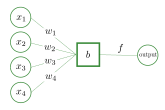
\includegraphics[width=0.6\columnwidth]{C4_cnn/neuron.pdf}
    \caption{Basic neuron}
    \label{machine:nn:neuron:plot}
\end{figure}

In the example in Fig.~\ref{machine:nn:neuron:plot} I have shows a neuron which has 4 input variables, or 4 input data points. 
When a network is trained, or when it learns, the weights applied to each of the inputs and the bias are updated to better represent the input data.
This training procedure is explained in more detail in Sec.~\ref{machine:nn:training}
Many neurons are then used in combination with each other to develop a neural network which can be applied to more complex problems.

%%%%%%%%%%%%%%%%%%%%
\subsection{\label{machine:nn:structure}Network structure}
%%%%%%%%%%%%%%%%%%%%

The structure of a neural network is defined by the user and there is no set way to design a network.
However, the general layout of a neural network is defined by structures called layers, sometimes known as fully connected layers. 
These are rows of $N$ neurons which all take the same input such that there is $N$ output values.
An example of a simple neural network is shown in Fig.~\ref{machine:nn:structure:plot}.
The first layer is the input layer, this is just the data points from an input example.
In the example of hand drawn digits, this would be the pixels from the image of the digit.
The final layer represents the information that you intend the network to extract from the input data. 
In the hand drawn digit example, this could have 10 output values corresponding to each digit 0-9. 
Each of these outputs is then a value which is related to the probability of that digit being present in the image.  

When designing a network, the user will have a defined input layer size from the data and a set number for the output layer which represents, for a classification example, the number of output classes. 
The number of hidden layers and the number of neurons in those hidden layers can be arbitrarily changed. 
In general if the data contains more complex information the size or complexity of the network will need to be increased for it to be able to extract the information. 
If there is a small number of training examples and a large and complex network, it may be able to learn the input data set as opposed the the general information that they represent.

\begin{figure}[h]
    \centering
    
\includegraphics[width=\columnwidth]{C4_cnn/simple_network.pdf}
    \caption{A neural network is structured with layers. Each of the circles in these layers are neurons as described in Sec.~\ref{machine:nn:neuron} and Fig.~\ref{machine:nn:neuron:plot}. The networks contain an input layer which is usually the data which you would like to analyse. Then this passes to a number of `hidden' layers, in the above diagram there are two. Hidden layers are just layers which exist between the input and the output. The output layer is then the desired output, above I have chosen a single neuron as output. This is such that the network could classify the input to a value between 0 and 1. Every neuron in a layer is connected to the output of all neurons in the previous layer.}
    \label{machine:nn:structure:plot}
\end{figure}


%%%%%%%%%%%%%%%%%
\subsection{\label{machine:nn:activation}Activation functions}
%%%%%%%%%%%%%%%%%

The activation function is how the output of a neuron is transformed. 
The most simple activation function is a cut as described in Sec.~\ref{machine:nn:neuron}, however, this type of activation does not perform well.
Activations functions a generally based on a few properties.
The activation function is generally non-linear, this allows networks with multiple layers to be used to approximate a function. A linear activation function means that any number of layers in a network is equivalent to a single layer network.
Another property which is desired in activation function is that it is continuously differentiable. This is to allow algorithms such as gradient descent to optimise the network. 
The functions are found to perform better if they are monotonic and smooth.
There are many choices when defining this in the network, some of the available options are shown in Fig.~\ref{machine:nn:activation:plot}.
One of the more commonly used activation function is the LeakyRELU function, this is explained in more detail in \citep{maas2013RectifierNonlinearities}.
In the work that follows we use the Leaky RELU function and the sigmoid function.


\begin{figure}[h]
	\centering
	\includegraphics[width=0.8\columnwidth]{C4_cnn/activations.pdf}
	\caption{There are many different activations function which are used, and essentially any function can be defined if necessary. Above is shown a subset of the more commonly used functions. The linear function is not used, however, is there to compare to common non linear function.}
	\label{machine:nn:activation:plot}
\end{figure}





%%%%%%%%%%%
%%%%%%%%%%%
\section{\label{machine:cnn}Convolutional Neural Networks}
%%%%%%%%%%%
%%%%%%%%%%%

\acp{CNN} are a different type of deep neural network than in Sec.~\ref{machine:nn}.
They are a types of network which are primarily used in image
processing and recognition
\cite{lecun2015DeepLearning,lecun1998GradientbasedLearning,waibel1989PhonemeRecognition,krizhevsky2012ImageNetClassificationa}.
Here the general idea is summarised. 
A \ac{CNN} is designed to take in data, identify different features within that data and classify
what those features or combinations of those features mean.
In the context of this work the input data is a time-frequency spectrogram which may contain a simulated \ac{CW} signal.
The output is then a single number which represents if a signal is present.
Here a value of 1 represents a signal and 0 is not a signal.
A \ac{CNN} can learn how to identify features by being trained on many
examples of the input data where the output is known.
For example, an input spectrogram with a simulated \ac{CW} signal would have an output value of 1.
Given the set of training examples, the many parameters of the \ac{CNN} can
be updated such that it gives the best result for any new image. 
This process is the same as neural networks in Sec.~\ref{machine:nn} and will be described in greater detain in Sec.~\ref{machine:training}

The key features of \acp{CNN} which distinguish them from ordinary neural networks is some additional types of layers including: Convolutional layers and max pooling layers. 


%%%%%%%%%%
%%%%%%%%%%
\subsection{Convolutional layers}
%%%%%%%%%%
%%%%%%%%%%

Convolutional layers have some similarities to standard fully connected layers as described in Sec.~\ref{machine:nn:structure}. 
The main difference being how the weights are applied to the inputs.
A fully connected neural network would flatten this image and apply Eq.~\ref{machine:nn:neuron:equation} to the inputs.
This involves having a separate weight for each of the input pixels in an image.
A convolutional layer however, filters the image and outputs a filtered image of the same size (the image can be a different size it depends how the layer was set up).
This convolution is defined by,
\begin{equation}
\label{machine:cnn:conv:equation}
O_{i,j} = f\left( \sum_{m} \sum_{n} F_{m,n}x_{i-m,j-n}\right) ,
\end{equation}
where $O$ is the output image, $x$ is the input image, $F$ is the convolutional filter and $f$ is the activation function.
The weights of the filter $F_{m,n}$ are what are updated when the network is trained.
Fig.~\ref{machine:cnn:convlayer:input} shows an example of a 6x6 image and the results of filtering the image using Eq.~\ref{machine:cnn:conv:equation} with two different filters $F$. 
In this case the network has 4 parameters for each filtered image which can be updated as opposed to the 36 which a full connected network would have for a single neuron.

Fig.~\ref{machine:cnn:convlayer:input} demonstrates how a filter which matches a feature in an image can highlight that particular feature. 
i.e. the diagonal line in the bottom left of the input is enhances by Filter 1, which matches that feature. 
When this type of layer is trained, the weights of the filter are updated. The filter should then ideally match the feature which is intended to be extracted.

\begin{figure}[p]

    \centering
    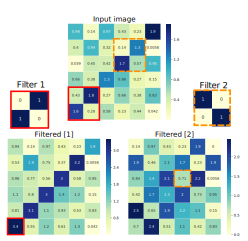
\includegraphics[width=\columnwidth]{C4_cnn/conv_filters.pdf}
    \caption{Convolutional filters can be designed to `pick out' certain features within an image. In this simple example above, the first filter (filter 1) matches the diagonal line in the bottom left of the input better than filter 2. The output filtered image the exaggerates this filter. The coefficients of the filter i.e. $F_{m,n}$ in Eq.~\ref{machine:cnn:conv:equation}, in this are set to ones and zeros.
    These are the weights which are trained by the network. In this an cases that follow, to get the same size image in the output as the input, the image is padded with zeros. I this image it was necessary to pad above and to the right of the image. The output of a convolutional layer is then the filtered images above after a bias and activation function have been applied. }
    \label{machine:cnn:convlayer:input}

\end{figure}

A convolutional layer has a number of different hyper-parameters which can be varied when setting up a model.
Below I list each of the adaptable parameters and what they do.

\begin{description}
\item[Filter size] The filter size is the size and shape of the convolutional filter. In Fig.~\ref{machine:cnn:convlayer:input} we use a filter size of 2$\times$2. The filter does not have to be square, however must be less than the dimensions of the image.

\item[Number of filters] The number of filters can be any value. If you have $K$ filter kernels, then the convolutional layer will output $K$ filtered images. In Fig.~\ref{machine:cnn:convlayer:input} we use two filters and therefore, the output of the layer is two images.

\item[Activation function] The activation function is generally kept the same for each of the layers, however this can be set here. The different types have been explained in Sec.~\ref{machine:nn:activation} and are applied as in Eq.~\ref{machine:cnn:conv:equation}.

\item[Stride] A normal convolutional layer applies a filter by multiplying by a filter, then shifting over by one pixel and repeating. Applying a stride mean rather than shifting by one pixel, one shifts by a number greater than one. This reduces the size of the output by the same factor of stride. i.e. if you skip one pixel (a stride of 2) then the image will be half the size on output. This has a similar affect to max-pooling which we describe in Sec.~\ref{machine:cnn:maxpool} an use for the rest of this work.  
\end{description}

The convolutional layers with reduce the number of updatable parameters used in each network or model.
However, the output of a convolutional layer is a number of images which ar potential the same size as the input. 
This has potentially increased the size of the parameter space for the next layer.
To decrease this a type of layer known as max-pooling is used.

%%%%%%%%%
%%%%%%%%
\subsection{\label{machine:cnn:maxpool}Max pooling layers}
%%%%%%%%%%%%
%%%%%%%%%%%

Max pooling layers are designed to reduce the size of the problem whilst holding on to as much important information as possible.
These do not contain any trainable parameters.
The idea of this layer is relatively simple, it reduces the image size by taking the maximum value in a region of a given size.
Fig.~\ref{machine:cnn:maxpool:image} shows the output of the first filtered image in Fig.~\ref{machine:cnn:convlayer:input}.
The image is then reduced by a 2$\times$2 max pooling layer.
The output of max-pooling Then shows a large value in the bottom left, this is where the input image matched the filter in Fig.~\ref{machine:cnn:convlayer:input}.
This demonstrates how the max-pooling layer can hold on to important information whilst reducing the image size.

\begin{figure}[h]
    \centering
    \includegraphics[width=\columnwidth]{C4_cnn/maxpool.pdf}
    \caption{Max pooling layers aim to reduce the size of am image whilst retaining important information within the original image. Above shows an example where a 2$\times$2 max-pooling layer is used on the output of Filter 1 in Fig.~\ref{machine:cnn:convlayer:input}. This retains the information that the input image matches the filter in the bottom left.}n
    \label{machine:cnn:maxpool:image}
\end{figure}

%%%%%%%%%%%%%
%%%%%%%%%%%%%%
\subsection{CNN structure}
%%%%%%%%%%%%%%
%%%%%%%%%%%%%%

\acp{CNN} are usually structured such that they can extract larger features from an input image, then the outputs from this are passed on to be classified.
The `feature extraction' part of the network consists of the convolutional layers and the max-pooling described in Sec.~\ref{machine:cnn}.
The outputs of the final max-pooling layer are then flattened and used as the input to a fully connected network.
This fully connected network the classifies these outputs into a number of classes.
Fig.~\ref{machine:cnn:structure:example} shows an example of the layout. 
Here an input image which is the same as in previous examples is passed onto a single convolutional layer with two different filters.
The output of two filtered images is passed to a max-pooling layer.
The two max-pooled images are flattened into 18 input neurons, this then passes through a fully connected network to a single output neuron.
This shows a simple example, however, there are many hyper-parameters of the network which can be changed.
These include: the number of filters in a convolutional layer, the number of convolutional layers and max-pooling layers, the number of hidden layers in the fully connected section and the number of neurons in the hidden layers. 
This example also shows the network being classified to a single output as this is how we use \acp{CNN} for the following work.

\begin{figure}[h]
	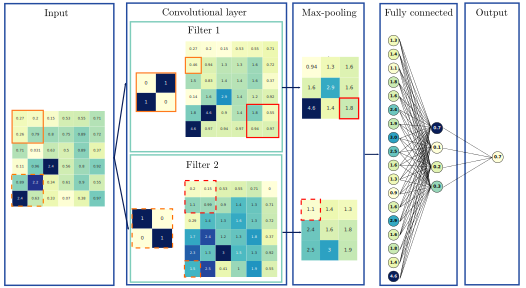
\includegraphics[width=\textwidth]{C4_cnn/cnn_structure_ex.pdf}
	\caption{Convolutional neural networks consist of two broad sections, the `feature extraction' part which is the convolutional and max-pooling layers, and the classification part which is the fully connected part of the network. This diagram shows a simple example of an image passing through a single convolutional layer with two filters, a single max-pooling layer and a simple fully connected network with a single hidden layer consisting of 4 neurons. }
	\label{machine:cnn:structure:example}
\end{figure}


%%%%%%%%%%%%%%%%%
\section{\label{machine:training}Training}
%%%%%%%%%%%%%%%%%

% introduce training concept
%
Once the structure of the network is decided, the network needs to be trained.
This means that the weights and bias' for every neuron and filter need to be updated such
that the neural network gives a useful output. For this
work we will classify the input images using a single output neuron.
This neuron outputs a value between 0 and 1 using a sigmoid function.
The \ac{CNN} is trained using a process called supervised
learning. When using supervised learning, the class of each input example is know. For example, we assign a label of 1 when the
input is a time-frequency spectrogram which includes a simulated \ac{CW}
signal. Similarly a time-frequency spectrogram with no simulated signal is assigned a label of 0. 
In general when training neural networks this way, the performance of the network can be improved by increasing the number of input examples which are shown to the network.
This stops the network from over-fitting to specific examples. Instead it should generalise to the full input and learn the underlying features within the data.

\subsection{Loss function}

%Training procedure
%
Each of the training examples is then propagated though the network to its single output value which lies between 0 and 1. Using a loss function, this output is then be compared to
the label of the input data which is either 0 or 1. There are many types of loss function which can be used, this depends on the type of problem which one wants to solve. As we are classifying
between two classes in out networks, the loss function, $L$, is the binary
crossentropy defined as,
%
\begin{equation}\label{cnn:loss} 
L = -y\log{(p)} + (1-y)\log{(1-p)},
\end{equation}
%
where $p$ is the networks predicted output which has any value in the range $[0,1]$ and $y$ is the true output which has binary labels 0 or 1. 
The loss function is minimised when the output matches the truth. This essentially
tells the neural network how close to the truth it is. The weights and bias' of
the neural network can be updated based on the value of this loss function. The
process of updating the weights and other parameters is called back-propagation,
and typically uses a form of gradient descent
\cite{kingma2015AdamMethod}.
Back-propagation uses the derivative of the loss function with respect to a weight to update that weight.
If changing that weight in a particular direction decreases the loss function, then the weight will be updated in that direction.
The size of the change of the weight value is related to the change in the size loss function.
This means that the weights can be updated to minimise the loss function and therefore improve the performance of the network.

%%%
%%%
\subsection{Training procedure}
%%%
%%%

The training procedure entails passing a set of training examples through the network a number of times. 
Once the entire training data set has been passed through the network (forward pass) and the weights have been updated accordingly (back propagation), the training has completed one epoch.
If the data was passed and the weights were updated a single time, the loss may decrease by is likely not at a minimum.
Passing the data through again may move the weights to a lower loss.
This process is repeated a number of times to try and find the minimum loss.

If for example the network is large, i.e. it has many trainable parameters, and the data set contains simple features, then the network can over train.
This mean the network learns specific features of the data-set rather than a general representation of it. 
To monitor this, after each epoch of training the loss is measured on a subset (test set) of the data which was not used for training. 
If the loss of the training set decreases but the loss of this test set begins to increase, then this is an indicator of over training. 

\joe{need to say somewhere what this actually does, i.e. why its useful}





%%%%%%%%%%%%%%%%%%%%%%%%%%%%%%%%%%%%%%%%%%%%%%
%%%%%%%%%%%%%%%%%%%%%%%%%%%%%%%%%%%%%%%%%%%%%%%%
\section{\label{machine:cw}Application to CW search}
%%%%%%%%%%%%%%%%%%%%%%%%%%%%%%%%%%%%%%%%%%%%%%%%%
%%%%%%%%%%%%%%%%%%%%%%%%%%%%%%%%%%%%%%%%%%%%%%%

The aim for this work is to use a \ac{CNN} to classify \ac{LIGO} data into one of two classes: signal or noise.
Here the signal class refers to a \ac{CW} signal from an isolated neutron star as described in Sec.~\ref{searchcw:model}.
Noise then refers to anything else which appear in the data, from Gaussian noise to instrumental artefacts. 
In Sec.~\ref{soap:results} to reduce the effect of instrumental artefacts, each of the search sub-bands was analysed by eye to determine if a sub-band was contaminated. 
Sub-bands which contained an artefact were then removed from the search.
This is a time consuming process. The main goal of the \ac{CNN} approach is to automate this part of the search.
This section will describe how we design the network to extract features and distinguish signals from instrumental artefacts.
We will then present results form searches in a range of \ac{LIGO} observing runs which include: S6, O1 and O2.


%%%%%%%%%%%%%%%
%%%%%%%%%%%%5%%
\subsection{\label{machine:cw:structure}Network structure}
%%%%%%%%%%%%%%%
%%%%%%%%%%%%%%%

In this section the structure of the networks which are used in this analysis
are described. There are three main inputs of data for each \ac{CNN}: spectrograms, Viterbi maps and the Viterbi statistic. Each of these are different representations of the raw detector data. In this analysis we train a separate \ac{CNN} for each of
these inputs and then a further three which use these combinations of inputs:
Viterbi map + spectrogram, Viterbi map + Viterbi statistic and Viterbi map +
Viterbi statistic + spectrogram. In all of the layers excluding the output layer of each \ac{CNN}, the activation functions in Eq.~\ref{machine:cnn:conv:equation} and \ref{machine:nn:neuron:equation} are defined by a function titled `leakyRELU' \cite{maas2013RectifierNonlinearities}. 
For our output neuron a sigmoid function is
used as an activation function such that the output is limited between 0 or 1.
For a given input a \ac{CNN} can then output a value between 0 and 1. When the output value is closer to 1, the input is more likely to contain a signal. 
The output value can then be treated as a detection statistic. 
The structure of the network is shown in Fig.~\ref{machine:results:cnnlayout} and is explained below. 

\begin{description}
	\item [Viterbi statistic] This is the simplest of the networks and will
	give the exact same result as the Viterbi statistic on its own. This is a
	single neuron which takes in the Viterbi statistic applies a weight and bias
	and then passes through a sigmoid function.
	
	\item [Viterbi map] The Viterbi map \ac{CNN} takes in a down-sampled Viterbi map of size (156,89), this is described more in Sec.~\ref{machine:data:downsample}.
	This \ac{CNN} consists of two convolutional layers and 3 fully connected layers. The first layer has
	8 filters which have a size of $5\times5$ pixels, the second layer has 8
	filters with a size of $3\times3$ pixels. After each of these layers we use a
	max-pooling layer with a size of $8\times8$ pixels. This then passed into three
	fully connected layers which all have 8 neurons and used leakyRELU activation
	functions. Finally these lead to an output neuron which uses a sigmoid
	function.
	
	\item [Spectrogram] The spectrogram \ac{CNN} takes in a down-sampled spectrograms of size (156,89), this is described more in Sec.~\ref{machine:data:downsample}.
	This \ac{CNN} has an identical structure as the Viterbi map \ac{CNN}, however, takes two channels as input. The two channels are the spectrograms of two different detectors.
	
\end{description}

The next three networks are constructed from combinations of the previous described \acp{CNN}.

\begin{description}
	\item [Viterbi map and spectrogram] To combine the spectrogram and Viterbi map network, we remove the final output neuron and its 8 weights from each of the networks. 
	The outputs from each network is then 8 neurons. These can be combined to a single sigmoid neuron which has 16 new weights.
	
	\item [Viterbi map and Viterbi statistic] In this network we combine the
	Viterbi statistic with the Viterbi map. As before, this uses the pre-trained
	Viterbi map and Viterbi statistic \acp{CNN}. The output sigmoid neuron and corresponding weights are removed from each network. 
	The 8 neurons from the Viterbi map network and the single neuron from the Viterbi statistic network are then combined to a single neuron with 9 new weights.
	
	\item [Viterbi map, Viterbi statistic and spectrogram] This combination takes all component \acp{CNN} from above. As before the final sigmoid output and the corresponding weights from each network are removed.
	The 8 neurons from the Viterbi map and spectrograms \acp{CNN} and the single neuron from the Viterbi statistic are then joined into a single output neuron with 17 new weights. 
	
\end{description}

When combining \acp{CNN} we use a process called transfer
learning~\cite{prattDiscriminabilityBasedTransfer}. This uses the pre-trained weights of the networks as a starting point to continue training. 
In our examples we found that we could fix the weights inside the pre-trained networks and just train the final 16 output weights from the neurons as in Fig.~\ref{machine:results:cnnlayout}.
These combinations of networks were chosen as the different representations of the data should contain slightly different information on the input.
For example, the Viterbi statistic contains no information on the structure of the track in the data and the Viterbi maps lost some information about lines in the band.
The addition of the spectrograms aimed to include even more information about this piece of data. 
Where when each of these are combined, the \ac{CNN} should be able to pick to important information from each of these representations.

% plot of vitmap and spretrogram structure 
%
\begin{figure}[p]
	\centering
	\includegraphics[width=0.9\columnwidth]{C4_cnn/networks.pdf}
	%
	\caption{\label{machine:results:cnnlayout} The structure of the Viterbi map and
		spectrogram \acp{CNN} used in this analysis are the same, with the difference
		that the spectrogram takes two images as input. They each use two convolutional
		layers and 3 fully connected layers before they're output to a single neuron which represents the probability of belonging to the signal class. The
		Viterbi statistic network is a single neuron that transforms the statistic into
		a number between 0 and 1 representing the probability of belonging to
		the signal class. For the combinations of networks, we remove the final
		output neuron and its 8 weights, i.e. we take the part inside the red or blue box. The 8 outputs from each network are then combined to a single neuron with 16 new weights. }
	%
\end{figure}


%%%%%%%%%%%%%%%%%%%%%%%%%%%%%%%%%%%%%%
%%%%%%%%%%%%%%%%%%%%%%%%%%%%%%%%%%%%%%
\section{\label{machine:data} Data generation}
%%%%%%%%%%%%%%%%%%%%%%%%%%%%%%%%%%%%%%
%%%%%%%%%%%%%%%%%%%%%%%%%%%%%%%%%%%%%%

% define the 3 data types that we consider
%

For the analysis that follows there are three main sets of data: training data,
testing data and search data. 
Training data is a set of data containing simulated signals which is used to train each of
the networks.
Test data is a separate set of simulations which is used to generate
efficiency curves and test the network.
Search data does not contain any simulated signal injections and is used to search for real signals.
For the majority of the analysis that follows, we use real detector data for all three of these data-sets, the exact observing runs will be explained in Sec.~\ref{machine:results}. 
The noise in real data contains many non Gaussian features, a particular class of these is known as instrumental lines and they have a large affect on \ac{CW} searches. 
The aim is to have a network which does not 
\joe{still trying to think how to write}
Each of these use
real data as it becomes difficult to simulate the many different classes of
instrumental line. The real data contains all the types of instrumental lines
which we need the network to identify.~\chris{this paragraph is a bit fluffy.
	Maybe say upfront that all data used is real detector data but then actually
	specify which real detector data O1,O2 etc... and give references. Also add a
	bit more about the detector lines. Maybe add that for each type of data you
	generate all 3 types of data product as defined in the previous section.} 

% describe the idea of odd and even bands
%
When training and testing a network it is important that the networks are not
trained and tested on the same data. Otherwise the \acp{CNN} can learn specific
features of the training data and not the underlying
distribution of features. To avoid this, the spectrograms are split into $0.1$
Hz wide sub-bands where alternating bands are designated as `odd' or `even'.
This means that bands starting with 100.1,100.3 are odd and 100.2,100.4 are
even etc. The networks can then be trained on the odd bands and tested on the
even bands and vice versa.
This then means that each time we want to search over data, we will have two final networks. One which will be run on odd bands and a separately trained network which is run on even bands. 

%%%%%%%%%%%%%%%%%%%%%%%%%%%%%%%%%%%%%%%%%%%%%%%%%%%%%%%
\subsection{\label{machine:data:injections} Signal simulations}
%%%%%%%%%%%%%%%%%%%%%%%%%%%%%%%%%%%%%%%%%%%%%%%%%%%%%%%

% describe signal injection
%
To inject the simulated signals into real data we generate a random set of signal
parameters which are drawn from prior distributions defined in
Table~\ref{machine:data:injections:table}. The \ac{SNR} of each simulation is then uniformly distributed between 50 and 150. Where the \ac{SNR} is the integrated `recovered' \ac{SNR}. This is calculated for each time segment using the definition of optimal \ac{SNR} in \cite{prix2007SearchContinuous}, the total \ac{SNR} is then the sum of the squares of these.
The \ac{GW} amplitude $h_{0}$ is scaled based on the noise \ac{PSD} to achieve this \ac{SNR}. 
The power spectrum of the signal can then be simulated in each time segment of a time-frequency spectrogram. This is done by assuming that the spectrogram is $\chi^2$ distributed.
The the antenna pattern functions are taken into account for the given source parameters and detector such that the \ac{SNR} for each time segment is calculated.
This \ac{SNR} is spread over neighboring frequency bins dependent on its location in frequency.
The power spectrum values can then be drawn from a non-central $\chi^2$ distribution with the non centrality parameter equal to the square of the \ac{SNR}.
Each signal is simulated in two detectors: \acp{LIGO} H1 and L1.
The \acp{SNR} reported below are then the sum of the squares of the \acp{SNR} from each detector.


% Table for simulated signal priors
%
\begin{table*}
	%                                         
	\caption{\label{machine:data:injections:table} Table shows the upper and lower limits
		over which each signal parameter was randomized. The parameters $\alpha,\sin{\left(\delta \right)},f,\;\log{\left( \dot{f} \right)},\; \cos{\left(\iota
			\right)},\; \phi_0,\; \psi$ were sampled
		uniformly in the ranges specified in the table. The frequencies $f_{\rm l}$ and $f_{\rm u}$
		refer to the lower and upper frequency of the band that each signal is injected
		into. Excluding the distribution of frequencies $f$, all the injections parameters are sampled from the same distributions as the S6
		\ac{MDC}~\cite{walsh2016ComparisonMethods}.}
	%
	\scalebox{0.9}{
	\bgroup
	\def\arraystretch{1.5}
	\centering
	\begin{tabular}{c c c c c c c c r|}
		\hline
		\hline
		& $\alpha$ [rad]& $\sin\left(\delta \right)$ [rad] & $f$ [Hz]&
		$\log_{10}\left(\dot{f} [\rm{Hz/s}]\right)$ & $\cos{\iota}$ [rad]& $\phi$ [rad]& $\psi$ [rad]\\
		\hline
		lower bound & $0$ & $-1$ & $f_{\rm l} + 0.25$ & $-9$ & $-1$ & $0$ & $0$ \\
		\hline
		upper bound & $2\pi$ & $1$ & $f_{\rm u} - 0.25$ & $-16$ & $1$ & $2\pi$ & $\pi/2$ \\
		\hline
	\end{tabular}
	\egroup
}	
\end{table*}

%%%%%%%%%%%%%%%%%%%%%%%%%%%%%%%%%%%%%%%%%%%%%%%%%%%
\subsection{\label{machine:data:augmentation} Augmentation}
%%%%%%%%%%%%%%%%%%%%%%%%%%%%%%%%%%%%%%%%%%%%%%%%%%%

% introduce augmentation
%
To train a neural network, many examples of data from each class are needed to avoid over-fitting.
In our case when we use data between 40-500 Hz, splitting the data into 0.1 Hz wide sub-bands does not give enough data for the
networks to be trained effectively. Therefore, using a technique called data
augmentation~\cite{patrice1991TangentProp,baird1992DocumentImage} we can
artificially increase the number of training examples.
Augmentation is when data is transformed such that, to the network, it appears to be `new'
data. 
For example, by shifting a time-frequency band up and down in frequency, this appears to be a new realisation of noise which we can then inject a simulated signal into.
This would double the size of the training data-set and reduce the likelihood of over-fitting to the training data. 

% exactly what we do for augmentation
%
The augmentations are applied to the spectrograms from each of the detectors.
The augmentations that are used on each sub-band are: reversing the data in
time, flipping the data in frequency, rolling the data in time by a small
number of segments and shifting the data in frequency by a small number of
bins. As we use real data, there are gaps in time where the detectors were not
operating. We preserve the location of these gaps when augmenting the data.
When shifting the data in frequency, we shift each band up and down by 30 frequency bins (0.016 Hz) and up and down by 60 frequency bins (0.032 Hz).
When rolling the data in time, we roll each sub-band by 100 time segments (100 days). 
Fig.~\ref{machine:data:augmentation:examples} shows examples of the original data, a flip in frequency, a roll in time and a flip in time.
For each frequency shift, we flip the sub-band in time and frequency and roll the sub-band in time.
This then gives us 3 transformations for each of the 4 frequency shifts, which including the original data gives 20 times the number of training examples.

\begin{figure}
	\centering
	\includegraphics[width=0.7\columnwidth]{C4_cnn/augmentation.pdf}
	\caption{The data is transformed by flipping the data in frequency (panel 2), rolling the data in time by 100 bins (panel 3) and flipping the data in time (panel 4). The original summed spectrogram is show in panel 1. Simulated signals can then be injected using this data as noise. The plots above show a broad wandering line to demonstrate the changes to the data when it is augmented, however, the majority of sub-bands contain almost Gaussian noise. }
	\label{machine:data:augmentation:examples}
\end{figure}

%%%%%%%%%%%%%%%%%%%%%%%%%%%%%%%%%%%%%%%%%%%%%%%%%
\subsection{\label{machine:data:downsample} Downsampling}
%%%%%%%%%%%%%%%%%%%%%%%%%%%%%%%%%%%%%%%%%%%%%%%%%

% introduce downsampling
%
One further issue for our data sets are their size. The spectrograms we use have a large number of pixels within them.
This means that as the spectrograms are passed through the network, there are a large number of computations.
Both this number of computations and the memory requirements of the GPU mean that training a network with a large number of data points takes longer.
We implement a few methods to reduce the size of the data: summing time segments of
spectrograms and down-sampling these summed spectrograms.  

% describe the downsampling in time and frequency
%
The spectrograms are summed over one day, i.e., every 48 time segments, as
in~\cite{bayley2019SOAPGeneralised}. This should increase the \ac{SNR} for a
given signal within a given time-frequency bin assuming that the
signal remains within the frequency bin for the majority of the time segment.
To reduce the size of the data further, the package `resize' from scikit-image
\cite{vanderwalt2014ScikitimageImage} is used, this uses interpolation to
resize the summed spectrograms to a size of (156,89) [time segments,frequency
bins]. This size was defined based on the summed spectrograms of the S6 data-set. This is 1/3 the number of summed segments in time, 1/2 the number of segments in frequency. The down-sampling is applied to the
spectrograms and vitmaps. 
In \cite{bayley2019SOAPGeneralised} we demonstrated that summing spectrograms can increase the speed and sensitivity of our search.
When down-sampling the image, we found that reducing the amount of data had a small affect on the sensitivity of the \acp{CNN} used.

%%%%%%%%%%%%%%%%%%%%%%%%%%%%%
%%%%%%%%%%%%%%%%%%%%%%%%%%%%%
\section{\label{machine:pipeline}Search pipeline}
%%%%%%%%%%%%%%%%%%%%%%%%%%%%%%%%%%%%
%%%%%%%%%%%%%%%%%%%%%%%%%%%%%%%%%

In previous sections each component of the search pipeline has been described,
however, described below is how each component fits together. Fig.~\ref{machine:pipeline:flow} shows a flow diagram of the pipeline. The pipeline is run in three different ways: training the \ac{CNN}, testing the search and running a search on real data. 

\begin{figure}[htp]
	\centering
	\scalebox{0.7}{
	

\tikzstyle{block} = [rectangle, draw, fill=blue!20, 
    text width=17em, text centered, rounded corners, minimum height=4em]
\tikzstyle{line} = [draw,line width=0.35mm, -latex']
\tikzstyle{fillnode} = [rectangle, fill=white, text centered]

\tikzstyle{blocktrain} = [rectangle, draw, fill=red!20, 
    text width=5em, text centered, rounded corners, minimum height=4em]
\tikzstyle{blocktest} = [rectangle, draw, fill=green!20, 
    text width=5em, text centered, rounded corners, minimum height=4em]
\tikzstyle{blocksearch} = [rectangle, draw, fill=black!5, 
    text width=5em, text centered, rounded corners, minimum height=4em]
\tikzstyle{blocktestbig} = [rectangle, draw, fill=green!20, 
    text width=17em, text centered, rounded corners, minimum height=4em]
\tikzstyle{blocksearchbig} = [rectangle, draw, fill=black!5, 
    text width=17em, text centered, rounded corners, minimum height=4em]
\tikzstyle{back group} = [fill=blue!20,rounded corners, draw=black!70, dashed, inner xsep=15pt, inner ysep=7pt, text centered]
\tikzstyle{back group1} = [fill=blue!20,rounded corners, draw=black!70, dashed, inner xsep=15pt, inner ysep=15pt, text centered]


\begin{tikzpicture}[node distance = 6em, auto]

    % Place node
    
  \node [block] (sft) {1.\\ SFTs from Time series};
  
  \node [block, below of=sft] (norm) {2. \\ Divide \ac{SFT} to running median and get power spectrum.};
  \node [block, below of=norm] (narrow) {3. \\ Narrowband \ac{SFT} };
  
  \node [block, below right =1.5cm and -0.9cm of narrow] (odd) {4. \\ Odd.};
  \node [block, below left =1.5cm and -0.9cm of narrow] (even) {4. \\ Even.};
  
  % odd blocks
    
  \node [blocktest,below of= odd] (testodd) {5b.\\ Test data};
  \node [blocktest, below of= testodd] (testsumodd) {6b. \\Test data};
  \node [blocktest, below of=testsumodd] (testlookupodd) {7b. \\ Test data};
  \node [blocktest, below of=testlookupodd] (testdownsampodd) {8b. \\  Test data};
  \node [below of= testdownsampodd](testblankodd) {};
    
  \node [blocktrain, left of= testodd] (trainodd) {5a.\\ Training data};
  \node [blocktrain, below of= trainodd] (trainsumodd) {6a. \\Training data};
  \node [blocktrain, below of=trainsumodd] (trainlookupodd) {7a. \\ Training data};
  \node [blocktrain, below of=trainlookupodd] (traindownsampodd) {8a. \\  Training data};
  \node [blocktrain, below of=traindownsampodd] (trainnetworkodd) {9. \\ Train `odd' \ \ac{CNN}};

  \node [blocksearch,right of=testodd] (searchodd) {5c.\\ Search data};
  \node [blocksearch, below of= searchodd] (searchsumodd) {6c. \\Search data};
  \node [blocksearch, below of=searchsumodd] (searchlookupodd) {7c. \\ Search data};
  \node [blocksearch, below of=searchlookupodd] (searchdownsampodd) {8c. \\  Search data};
  \node [below of= searchdownsampodd](searchblankodd) {};
  
  \node [blocktest, below = 1.4cm of testblankodd] (testclassifyodd) {10b.\\ Test data};
  \node [blocksearch, below = 1.4cm of searchblankodd] (searchclassifyodd) {10c.\\ Search data};

   
  % even blocks]
  
    \node [blocksearch,below of=even] (searcheven) {5c.\\ Search data};
  \node [blocksearch, below of= searcheven] (searchsumeven) {6c. \\Search data};
  \node [blocksearch, below of=searchsumeven] (searchlookupeven) {7c. \\ Search data};
  \node [blocksearch, below of=searchlookupeven] (searchdownsampeven) {8c. \\ Search data};
  \node [below of= searchdownsampeven](searchblankeven) {};
  
  \node [blocktest,left of= searcheven] (testeven) {5b.\\Test data};
  \node [blocktest, below of= testeven] (testsumeven) {6b. \\Test data};
  \node [blocktest, below of= testsumeven] (testlookupeven) {7b. \\Test data};
  \node [blocktest, below of=testlookupeven] (testdownsampeven) {8b. \\ Test data};
  \node [below of= testdownsampeven](testblankeven) {};
  
  \node [blocktrain, right of= searcheven] (traineven) {5a.\\ Training data};
  \node [blocktrain, below of= traineven] (trainsumeven) {6a. Training data};
  \node [blocktrain, below of=trainsumeven] (trainlookupeven) {7a. \\Training data};
  \node [blocktrain, below of=trainlookupeven] (traindownsampeven) {8a. \\ Training data};
  \node [blocktrain, below of=traindownsampeven] (trainnetworkeven) {9. \\ Train `even'  \ \ac{CNN}};

  
  \node [blocktest, below = 1.4cm of testblankeven] (testclassifyeven) {10b.\\ Test data};
  \node [blocksearch, below = 1.4cm of searchblankeven] (searchclassifyeven) {10c.\\ Search data};
  
% background blocks  
  
\begin{scope}[on background layer]
   
    \node (bkgen) [back group] [fit=(trainodd) (testodd) (searchodd) (traineven) (testeven) (searcheven) ] {5.\\Injections};
    
    \node (bksum) [back group] [fit=(trainsumodd) (testsumodd) (searchsumodd) (trainsumeven) (testsumeven) (searchsumeven)] {6.\\Sum spectrograms over \\1 day};
    
    \node (bksoap) [back group] [fit=(trainlookupodd) (testlookupodd) (searchlookupodd) (trainlookupeven) (testlookupeven) (searchlookupeven)] {7.\\Generate lookup tables \\and\\ run SOAP search.};
    
    \node (bkdown) [back group] [fit=(traindownsampodd) (testdownsampodd) (searchdownsampodd) (traindownsampeven) (testdownsampeven) (searchdownsampeven)] {8.\\Downsample spectrograms\\ and vitmaps.};
    
    \node (bkclassodd) [back group1] [fit=(testclassifyodd) (searchclassifyodd)] {};
     
    \node (bkclasseven) [back group1] [fit=(testclassifyeven) (searchclassifyeven)] {};

    
 \end{scope}
 
   % search and testing
  
  \node [blocktestbig, below right =1.1cm and -3.5cm of bkclasseven] (output) {11c.\\ Generate efficiency curves from test data.};
  \node [blocksearchbig, below left= 1.1cm and -3.5cm of bkclassodd] (outputsearch) {11a.\\ Take top 1\% of search bands for followup.};
  
  % Draw edges
  \path [line] (sft) -- (norm);
  \path [line] (norm) -- (narrow);
  
  % even lines
  
   \path [line] (narrow) -- (even);
  
  \path [line] (even) -- (testeven);
  \path [line] (even) -- (traineven);
  \path [line] (even) -- (searcheven);
  
  \path [line,red!60] (traineven) -- (trainsumeven.north);
  \path [line,green!60] (testeven.south) -- (testeven.south|-testsumeven.north);
  \path [line,black!60] (searcheven.south) -- (searcheven.south|-searchsumeven.north);
  
  \path [line,green!60] (testeven.south|-testsumeven.south) -- (testeven.south|-testlookupeven.north);
  \path [line,red!60] (traineven.south|-trainsumeven.south) -- (traineven.south|-trainlookupeven.north);
  \path [line,black!60] (searcheven.south|-searchsumeven.south) -- (searcheven.south|-searchlookupeven.north);
  
  \path [line,green!60] (testeven.south|-testlookupeven.south) -- (testeven.south|-testdownsampeven.north);
  \path [line,red!60] (traineven.south|-trainlookupeven.south) -- (traineven.south|-traindownsampeven.north);
  \path [line,black!60] (searcheven.south|-searchlookupeven.south) -- (searcheven.south|-searchdownsampeven.north);
  
  \path [line,red!60] (traindownsampeven) -- (trainnetworkeven);
  \path [line,green!60] (testdownsampeven) -- (testclassifyeven);
  \path [line,black!60] (searchdownsampeven) -- (searchclassifyeven);
  
  %\path [line,black!60] (searcheven.south|-searchdownsampeven.south) -- (searcheven.south|-classifyeven.north);
  %\path [line,green!60] (testeven.south|-testdownsampeven.south) -- (testeven.south|-classifyeven.north);
  
  \path [line,red!60] (trainnetworkeven) -- (bkclassodd);
  
  %% odd lines
  
   \path [line] (narrow) -- (odd);
  
  \path [line] (odd) -- (testodd);
  \path [line] (odd) -- (trainodd);
  \path [line] (odd) -- (searchodd);
  
  \path [line,red!60] (trainodd) -- (trainsumodd.north);
  \path [line,green!60] (testodd.south) -- (testodd.south|-testsumodd.north);
  \path [line,black!60] (searchodd.south) -- (searchodd.south|-searchsumodd.north);
  
  \path [line,green!60] (testodd.south|-testsumodd.south) -- (testodd.south|-testlookupodd.north);
  \path [line,red!60] (trainodd.south|-trainsumodd.south) -- (trainodd.south|-trainlookupodd.north);
  \path [line,black!60] (searchodd.south|-searchsumodd.south) -- (searchodd.south|-searchlookupodd.north);
  
  \path [line,green!60] (testodd.south|-testlookupodd.south) -- (testodd.south|-testdownsampodd.north);
  \path [line,red!60] (trainodd.south|-trainlookupodd.south) -- (trainodd.south|-traindownsampodd.north);
  \path [line,black!60] (searchodd.south|-searchlookupodd.south) -- (searchodd.south|-searchdownsampodd.north);
  
  \path [line,red!60] (traindownsampodd) -- (trainnetworkodd);
  \path [line,green!60] (testdownsampodd) -- (testclassifyodd);
  \path [line,black!60] (searchdownsampodd) -- (searchclassifyodd);
  
  %\path [line,black!60] (searchodd.south|-searchdownsampodd.south) -- (searchodd.south|-classifyodd.north);
  \%path [line,green!60] (testodd.south|-downsampodd.south) -- (testodd.south|-classifyodd.north);
  
  \path [line,red!60] (trainnetworkodd) -- (bkclasseven);
  
  % search and test
  
  \path [line,green!60] (testclassifyeven) -- (output);
  \path [line,black!60] (searchclassifyeven) -- (outputsearch);
  
  \path [line,green!60] (testclassifyodd) -- (output);
  \path [line,black!60] (searchclassifyodd) -- (outputsearch);
  
  % final labels over lines
  
   \node[fillnode,below] at (bkclasseven.south) {Classify sub-bands with \ `odd' \ac{CNN}};
   
   \node[fillnode,below] at (bkclassodd.south) {Classify sub-bands with \ `even' \ac{CNN}};
 
    
\end{tikzpicture}}
	\caption{\label{machine:pipeline:flow} This diagram shows the SOAP pipeline from start to finish. There are three main sections: Training (red), Testing (green) and Searching (grey) for both the odd and even bands. The blue sections mean that the same operations is done in all cases.}
	
\end{figure}

\begin{description}
	\item[1. \acp{SFT}] Generate 1800s long \acp{SFT} from detector time-series data. For this search these are already generated.
	
	\item[2. Normalising] The \acp{SFT} are then divided by their running median such that their power spectrum has a mean of $\sim 1$. Each spectrogram is then multiplied by 2 such that they are approximately $\chi^{2}$ distributed.
	
	\item[3. Narrowbanding] To improve the computational efficiency of the search the spectrograms are split into 
	$2.1$ Hz wide bands every $2$ Hz,
	i.e. 100.0-102.1, 102.0-104.1 etc.
	This band size was chosen based on the available computational memory at the time.
	
	\item[4. Band splitting]  As a \ac{CNN} should not be trained on the same data that it will be tested on, each of the $0.1$ Hz wide sub-bands are split into `odd' or `even' bands. 
	
	\item[5a. Training data generation] To generate training data the
	process is the same as in Sec.~\ref{data}.  Each of the $0.1$ Hz sub-bands is `augmented' as in Sec.~\ref{machine:data:augmentation}. For each of the augmented bands, the data is duplicated and then signals are injected into them with \acp{SNR} in the range 50-150. This gives us and example for a noise class and a signal class. There are two of these sets, on for `even' bands and one for `odd'.
	
	\item[5b. Test data generation] For test data signals following parameters in Tab.~\ref{machine:data:injections:table} are injected in to 50\% of the $0.1$ Hz sub-bands. These signal have and \ac{SNR} in the range 20-200. Where we have a set for `odd' and a set for `even'.
	
	\item[5c. Search data] This data is generated such that we can search for a real signal. The sub-bands described in part 4 are now overlapping by 0.05 Hz. This means that if there is a signal it should be fully contained within at least one sub-band. There are both `odd' and `even' versions of this search data.
	
	\item[6. Summing spectrogram] As in \cite{bayley2019SOAPGeneralised} the spectrograms are summed over one day, i.e. every 48 time segments of the spectrogram are summed. This is done separately for each of the 6 data-sets (3 for `odd', 3 for `even'). 
	
	\item[7. Generate lookup tables and run SOAP search] Before the SOAP search is run, the line-aware statistic lookup tables need to be generated as in \cite{bayley2019SOAPGeneralised}. Then for each of the 6 data-sets (3 for `odd', 3 for `even') the SOAP search is run separately. 
	
	\item[8. Down-sample data] At this stage there are four elements which are saved for each of the 6 data-sets. The two spectrograms, the Viterbi maps and the Viterbi statistic. The spectrograms and the Viterbi maps are down-sampled to a size of (156x89) using interpolation from scikit-image's resize \cite{vanderwalt2014ScikitimageImage}. This size was chosen based on the S6 \ac{MDC} data-set, where this is 1/3 the length in time and 1/2 the width in frequency of the summed spectrograms.
	
	\item[9. Train Networks] The down-sampled training data is then used to train a \acp{CNN}. One \ac{CNN} is trained on `odd' bands and a different \ac{CNN} with the same structure is trained `even' bands. 
	
	\item[10b. Run search on test data] The trained \acp{CNN} from part 9 are then used to classify each sub-band in the test data with injections, this returns a statistic in $[0,1]$ where 1 represents the probability of a signal. Here the \ac{CNN} trained on the `odd' bands is tested using the `even' bands and vice versa.
	
	\item[10c. Run search on real data] The trained \acp{CNN} from part 9 are then used to classify each sub-band in the search data, this returns a statistic in $[0,1]$ where 1 represents the probability of a signal. Once again the \ac{CNN} trained on the `odd' bands is tested using the `even' bands and vice versa.
	
	\item[11a. Signal candidates] The signals which have a statistic in the top 1\% are taken for a followup investigation. This can be another search, or just a look `by-eye'.
	
	\item[11c. Efficiency curves] The statistics can be plotted against \ac{SNR} to see how the network classified signals with the \ac{SNR} of the injection. Then the efficiency curves can be generated, this is described in further detail in Sec.~\ref{machine:results:sensitivity} .
	
	
	
\end{description}


%%%%%%%%%%%%%%%%%%%%%%%%%%%%
%%%%%%%%%%%%%%%%%%%%%%%%%%%%
\section{\label{machine:results}Results}
%%%%%%%%%%%%%%%%%%%%%%%%%%%%
%%%%%%%%%%%%%%%%%%%%%%%%%%%%

The networks described in Sec.~\ref{machine:cnn:networks} were trained and tested on four different data-sets: the S6 \ac{MDC} as in \cite{bayley2019SOAPGeneralised,walsh2016ComparisonMethods}, our own injections into O2 data and Gaussian noise which had the same gaps and noise floor as the S6 data-set, and our own injections into real S6 data. 
Each of the searches use training and test data in the frequency range of 100-400 Hz, except the S6 \ac{MDC} which uses data in the range 40-500 Hz for testing and training. 


\subsection{\label{machine:results:sensitivity} Sensitivity}

To investigate the sensitivity of the pipeline we use two measures: the sensitivity depth $\mathcal{D}$ \cite{prix2007SearchContinuous} and optimal \ac{SNR} $\rho$ \cite{behnke2015PostprocessingMethods} which are both defined in \cite{bayley2019SOAPGeneralised} as,
%
\begin{equation}
\label{sigmoid}
\mathcal{D}(f) = \frac{\sqrt{S_h(f)}}{h_0},
\end{equation}
%
where $S_h(f)$ is the single-sided noise \ac{PSD} and $h_0$ is the \ac{GW} amplitude. The optimal \ac{SNR} is defined as,
%
\begin{equation}
\rho^2 = \sum_X 4
\Re\int^{\infty}_{0}\frac{\tilde{h}^X(f)\tilde{h}^{X*}(f)}{S^X(f)}df,
\end{equation}
%
where $X$ indexes the detectors and $\tilde{h}(f)$ is the Fourier transform of the time series of the signal $h(t)$. 
This expression is defined in~\cite{prix2007SearchContinuous} for a double-sided \ac{PSD} and we have defined it for the more common single-sided case.

The sensitivity curves shown in Fig.~\ref{results:o2},\ref{results:s6gauss} and \ref{results:s6mdc} were generated using a $1\%$ false alarm rate, where the false alarm is the value where $1\%$ of bands which do not contain an injection exceed the false alarm. 
This is then used as a detection threshold, such that the statistics for each band which exceed this threshold are converted to a 1 and all that do not to a 0.
From this point we use a window to estimate the efficiency curve for each \ac{SNR}, this follows,
\begin{equation}
y(x) = \frac{\sum_i b_i \mathcal{G}(x_i - x,2)}{\sum_i \mathcal{G}(x_i - x,2)},
\end{equation}
where $b_i$ is the binomial data where $b_i=1$ when the statistic is above the $1\%$ false alarm value, $x_i$ is the \ac{SNR} of point $b_i$, $x$ is the current location in \ac{SNR} and $\mathcal{G}(x_i - x,2)$ is a Gaussian with a mean of the current \ac{SNR} and a standard deviation of 2.
The efficiency curves for each of the described data-sets are shown in Figs.~\ref{results:o2},\ref{results:s6gauss} and \ref{results:s6mdc}.


%%%%%%%%
\subsubsection{O1}
%%%%%%%%%%

For the first test, injections were made into the O1 data-set as in Sec.~\ref{data} between 100 Hz and 400 Hz. Then each of the 6 networks described in Sec.~\ref{cnn:networks} were trained and tested on this data. 
Fig.~\ref{machine:results:o1} shows the sensitivity curves for this test for both \ac{SNR} and sensitivity depth for each of the 6 networks. Focusing on Fig.~\ref{machine:results:snr_o1}, the least sensitive, i.e. furthest to the right, of the \acp{CNN} is the Viterbi statistic (vitstat), this is expected as we know that the Viterbi statistic is sensitive to instrumental lines. 
The spectrogram \ac{CNN} has an improved sensitivity over the Viterbi statistic, this importantly does not involve the SOAP search but is run entirely on down-sampled and summed spectrograms. 
Whilst this network is approaching the most sensitive of the examples in Fig.~\ref{results:o2}, and with further efforts may reach it, this network takes $\sim10$ times the amount of training time. This will be explained in more detail in Sec.~\ref{results:timing}.
The remaining networks achieved almost the same sensitivity. 
The vitmap network however, is the fastest of these to train and is used as an input for all of these remaining networks.
For the O1 data-set we show that with a false alarm of 1\% the Viterbi map \ac{CNN} achieves a sensitivity of SNR $~73$ and sensitivity depth of $~12\; {\rm Hz}^{-1/2}$ with 95\% efficiency.
The \ac{SNR} here should not be compared between different runs as this is the integrated `Recovered' \ac{SNR}. Therefore, observing runs, such as O1, which were shorted will appear to have a greater sensitivity when they in fact do not. 

\begin{figure}
	%\centering
	\begin{subfigure}[h]{0.5\textwidth}
		\includegraphics[width=\columnwidth]{C4_cnn/o1_snr_eff.pdf}
		\label{machineresults:snr_o1}
	\end{subfigure}
	\begin{subfigure}[h]{0.5\textwidth}
		\includegraphics[width=\columnwidth]{C4_cnn/o1_depth_eff.pdf}
		\label{machine:results:depth_o1}
	\end{subfigure}
	\caption{\label{machine:results:o1} In the O1 data-set, each of the six \acp{CNN} were tested. The efficiency plots above are for a 1\% false alarm rate.  }
	
\end{figure}

%%%%%%%%%
\subsubsection{O2}
%%%%%%%%%%

For the next test, injections were made into the O2 data-set in the same way as in the last section. Then each of the 6 networks described in Sec.~\ref{cnn:networks} were trained and tested on this data. 
Fig.~\ref{machine:results:o2} shows the sensitivity curves for this test for both \ac{SNR} and sensitivity depth for each of the 6 networks.
The results here are very similar to the results from the O1 simulations.
The Viterbi statistic is the least sensitive `network', followed by the spectrogram \ac{CNN}.
The remaining four networks all achieve a similar sensitivity, each of these remaining networks contain the Viterbi map as one of their inputs. Therefore, it is assumed that the dominating effect on the sensitivity originated from the Viterbi maps. In following tests the focus will be with the Viterbi map \ac{CNN} as in all cases this is among the most sensitive.
For the O2 data-set we show that with a false alarm of 1\% the Viterbi map \ac{CNN} achieves a sensitivity of SNR $~95$ and sensitivity depth of $~12\; {\rm Hz}^{-1/2}$ with 95\% efficiency.
This result in the sensitivity depth in Fig.~\ref{machine:results:depth_o2} does not vary much from the results from O1, Fig.~\ref{machine:results:depth_o1}. 
Whilst one might expect the sensitivity to increase due to the increase in sensitivity and longer observing run.
However, this is not the case \joe{why?}.

\begin{figure}
	%\centering
	\begin{subfigure}[h]{0.5\textwidth}
		\includegraphics[width=\columnwidth]{C4_cnn/o2_snr_eff.pdf}
		\label{machine:results:snr_o2}
	\end{subfigure}
	\begin{subfigure}[h]{0.5\textwidth}
		\includegraphics[width=\columnwidth]{C4_cnn/o2_depth_eff.pdf}
		\label{machine:results:depth_o2}
	\end{subfigure}
	\caption{\label{machine:results:o2} In the O2 data-set, each of the six \acp{CNN} were tested. The efficiency plots above are for a 1\% false alarm rate. These show that the use of spectrograms and the Viterbi maps with \acp{CNN} greatly improve the sensitivity when compared to the Viterbi statistic. For each \ac{CNN} which uses a combination of inputs it achieves a similar sensitivity to the \ac{CNN} which uses just the Viterbi map. This implies that the Viterbi map contains the most information out of the tested \acp{CNN}. }
	
\end{figure}



%%%%%%%%%
\subsubsection{Gaussian noise}
%%%%%%%%%%%

The next test involves using injections into Gaussian noise. For this test we tried to replicate the S6 data-set without including instrumental artefacts such as lines. We included the same gaps in data as S6 and the noise floor of S6 was replicated by scaling the \ac{SNR} of any injection in any given \ac{SFT}. 
Fig.~\ref{machine:results:s6gauss} shows the sensitivity curves for the Viterbi statistic and Viterbi map \ac{CNN} for both the Gaussian noise run with S6 gaps and for injections into the S6 data-set. 
In the Gaussian noise data-set the curves for both statistics, Viterbi map and the Viterbi statistic, show very similar results, this is to be expected as the main use of the \ac{CNN} was to reduce the effect of instrumental lines, for which there is none in this data set. 
The advantage of using the Viterbi maps in a \ac{CNN} becomes clear which it is tested on injections into real data with many instrumental lines. 
The remaining curves in Fig.~\ref{machine:results:s6gauss} show these tests, and it becomes clear that the Viterbi map \ac{CNN} reduces the effect of instrumental lines and therefore increases the searches sensitivity. 
These tests in S6 also show that the effect of instrumental lines was far greater in this run than in O2. 
This is shown in Fig.~\ref{machine:results:o2} where the separation between the Viterbi statistic curves and the Viterbi map curves is much smaller than the S6 curves in Fig.~\ref{machine:results:s6gauss}.
For injections into Gaussian noise following S6 gaps we show that with a false alarm of 1\% the Viterbi map \ac{CNN} achieves a sensitivity of SNR $~85$ and sensitivity depth of $~20\; {\rm Hz}^{-1/2}$ with 95\% efficiency. For injections into real S6 data the search achieves a sensitivity of SNR $~115$ and sensitivity depth of $~11\; {\rm Hz}^{-1/2}$ with 95\% efficiency and 1\% false alarm. We can also see from Fig.~\ref{machine:results:s6gauss} that the sensitivity in Gaussian noise with S6 gaps is better than in real S6 data, so there are still some elements of the search which reduces the sensitivity.

\begin{figure}
	\begin{subfigure}[h]{0.5\textwidth}
		\includegraphics[width=\columnwidth]{C4_cnn/gauss_and_s6_snr_eff.pdf}
		\label{machine:results:snr_s6}
	\end{subfigure}
	\begin{subfigure}[h]{0.5\textwidth}
		\includegraphics[width=\columnwidth]{C4_cnn/gauss_and_s6_depth_eff.pdf}
		\label{machine:results:depth_s6}
	\end{subfigure}

	\caption{\label{machine:results:s6gauss} We aimed to compare the sensitivity of this search on simulations on real data (s6) to simulations in Gaussian noise (gauss). The Gaussian noise injections included the same gaps in data as the S6 data set. The \ac{SNR} of the simulated signal in Gaussian noise was adjusted based on the noise floor of S6. The sensitivity curves show that the Viterbi map \ac{CNN} (vitmap)achieves a similar sensitivity to the Viterbi statistic (vitstat) in Gaussian noise. This is because the main factor which effects the sensitivity of the Viterbi statistic is instrumental lines. As expected in real data, the Viterbi statistic is far less sensitive. The power of the \ac{CNN} becomes clear in tests on real data. The sensitivity of the Viterbi map \ac{CNN} is improved by over a factor of 2 in \ac{SNR} when tested on S6 data.}
	
\end{figure}

%%%%%%%
\subsubsection{S6}
%%%%%%%%%%

The final test was set up to again use the S6 data-set, however, we use a standard set of injections in the S6 \ac{MDC} \cite{walsh2016ComparisonMethods} to compare directly to other \ac{CW} search pipelines. In Fig.~\ref{machine:results:s6mdc} we show the results of the sensitivity curves from these injections. Fig.~\ref{machine:results:mdccomp} shows the direct comparison in depth of the results in \cite{walsh2016ComparisonMethods} with the results from the SOAP search with the Viterbi map \ac{CNN}. This shows that we achieve a sensitivity similar to many other semi-coherent searches with the exception of the Einstein@home search \cite{abbott2016ResultsDeepest}. For tests in the S6 \ac{MDC} we show that with a false alarm of 1\% the Viterbi map \ac{CNN} achieves a sensitivity of SNR $~90$ and sensitivity depth of $~16\; {\rm Hz}^{-1/2}$ with 95\% efficiency.


\begin{figure}
	\begin{subfigure}[h]{0.5\textwidth}
		\includegraphics[width=\columnwidth]{C4_cnn/S6MDC_snr.pdf}
		\label{machine:results:snr_s6mdc}
	\end{subfigure}
\begin{subfigure}[h]{0.5\textwidth}
	\includegraphics[width=\columnwidth]{C4_cnn/S6MDC_depth.pdf}
	\label{machine:results:mdccomp}
\end{subfigure}

	\caption{\label{machine:results:s6mdc} In the S6 \ac{MDC} \cite{walsh2016ComparisonMethods}, sensitivity curves were made for a set of \ac{CW} searches. 
		We have taken the list of detected pulsars for each search from this paper \cite{walsh2016ComparisonMethods} and replotted using the method in Sec.~\ref{sensitivity} to compare the sensitivities. 
		This is results for all pulsar injections in the 40-500 Hz band in the S6 \ac{MDC}.
		This shows how the SOAP search with a \ac{CNN} achieves a similar sensitivity some other \ac{CW} searches. 
	}
	
\end{figure}


\subsection{\label{results:timing} Computational time}

A key part of any \ac{CW} search is the computational time taken, the majority of the time for this search is used generating the appropriate data. 
For each section of the pipeline we have take the average total time for each job to complete, where each job runs on 2.0 Hz and it runs between 100 and 400 Hz. These are approximate timings taken for all the jobs to finish when run on CIT and can vary.

\begin{table}[h]
	%                     
	\centering                                                                                            
	\caption{\label{timing:table}Table shows the timings for each part of the search. These are approximate timings and vary when different amounts of data are input. This was run on data between 100-400 Hz.}
	
	%   
	\scalebox{0.8}{%
	\bgroup
	\def\arraystretch{1.5}
	\centering
	\begin{tabular}{c c c}
		\multicolumn{3}{c}{{\bf Generating data on CPU}}  \\
		\hline
		\hline
		& Time [hrs] & \\
		\hline
		Narrow-banding & $9$ &  \\
		\hline
		Training data& $239$ & \\
		\hline
		Test data& $75$ & \\
		\hline
		Search data& $40$ & \\
		\hline
		\hline
		\multicolumn{3}{c}{{\bf Training \acp{CNN} on GPU} }  \\
		\hline
		\hline
		& Training time [hrs] & Loading time [hrs]\\
		\hline
		Viterbi statistic & $0.03$ & $0.2$ \\
		\hline
		Viterbi map & $0.8$ & $0.7$ \\
		\hline
		spectrogram & $9$ & $1$\\
		\hline
		Viterbi map \\ + Viterbi statistic& $1$ &$0.7$ \\
		\hline
		Viterbi map \\ + spectrogram& $1.4$ & $1.6$\\
		\hline
		Viterbi map \\ + Viterbi statistic \\ + spectrogram& $1.5$ & $2$ \\
		\hline
		\hline
		\multicolumn{3}{c}{{\bf Testing \acp{CNN} on real data on GPU}}  \\
		\hline
		\hline
		& Testing [s] & Loading [s] \\
		\hline
		& $5$ & $60-160$ \\
		\hline
		\hline
	\end{tabular}
	\egroup
}
\end{table}

This gives the entire search including testing a total run time of $ \sim 386$ hours, however, the majority of the time is taken generating data which can be easily parallelised. 
Rather than taking hundreds of hours, the generating data sections takes $\mathcal{O}(1)$ hours in real time.


%%%%%
%%%%%
\section{\label{machine:cnn:sens_size} Sensitivity with the size of dataset}
%%%%%
%%%%%

When training a network, the general rule is the more data the better. 
This limits effects such as over-training mentioned in Sec.~\ref{machine:nn:training}.
To investigate how the sensitivity of the search changes with the number of training examples, the Viterbi map (vitmap) network in Sec.\ref{machine:results} was trained using a range of different training example numbers. 
These networks are then tested on the same dataset to see how they perform.
This was repeated for two data-sets: \ac{CW} simulations in Gaussian noise and simulations in \acp{LIGO} O1 data-set. 
For both of these cases six different networks were trained, these used 100, 500, 1000, 5000, 10000 and 15000 Viterbi maps as their training datasets.
Here the training data-sets are the same used as in Sec.~\ref{}.
These were then tested on the same data-sets in Sec.~\ref{}.

In the Gaussian noise case, the majority of the networks performed the same. 
This is with the exception of the network which was trained with 100 input Viterbi maps. 
The implication of this is that the information in the Viterbi maps is relatively easy to extract in this case. 
As the network is trying to distinguish Gaussian noise from a simulated \ac{CW} signal, one would expect this to be the easiest of all examples above to solve. \joe{dont like this explanation}

\begin{figure}[h]
	\begin{subfigure}[h]{0.5\textwidth}
		\includegraphics[width=\linewidth]{C4_cnn/gauss_sens_with_trainnum_eff.pdf}
		\caption{}
	\end{subfigure}
	\begin{subfigure}[h]{0.5\textwidth}
		\includegraphics[width=\linewidth]{C4_cnn/gauss_sens_with_trainnum.pdf}
		\caption{}
	\end{subfigure}
	\caption{}
	\label{machine:cnn:sens_size:gauss_sens}
\end{figure}

When simulating signals in real O1 data, many of the sub-bands will contain instrumental lines. 
The noise class for the networks then contains many variations compared to the Gaussian noise case. 
This a harder challenge to the neural network by essentially increasing the size of the parameter space.
Because of this, one would expect the network to need many more training examples to be able to achieve a similar sensitivity to Gaussian noise.
In Fig.~\ref{machine:cnn:sens_size:o1_sens}, one can see that using 100 training examples is not enough and the network does not achieve any sensitivity at any \ac{SNR}.
The increase in training examples has a larger affect than in the Gaussian noise case. \joe{is that true}



\begin{figure}[h]
	\begin{subfigure}[h]{0.5\textwidth}
		\includegraphics[width=\linewidth]{C4_cnn/o1_sens_with_trainnum_eff.pdf}
		\caption{}
	\end{subfigure}
	\begin{subfigure}[h]{0.5\textwidth}
		\includegraphics[width=\linewidth]{C4_cnn/o1_sens_with_trainnum.pdf}
		\caption{}
	\end{subfigure}
	\caption{}
	\label{machine:cnn:sens_size:o1_sens}
\end{figure}



%%%%%%%%%%%
%%%%%%%%%%%
\section{\label{cnn:networkvis}Network Visualisation}
%%%%%%%%%%%
%%%%%%%%%%%

Neural network are generally hard to visualise due to the large number or parameters in the network that have to be varied.
However, there are methods which can be used to see how input data is affected by the network.
This can be useful to see how the network performs when given certain types of data and gives some insight into how the networks work

In the examples above we use \acp{CNN}, the first few layers of this are build using convolutional filters.
The filters weights should ideally correspond to the shape of the feature which one wants to extract from the image. 
Generally this is only useful to picture at the first layer as the network can make subsequent layer and representations quite abstract.



\begin{figure}[h]
	\centering
	\includegraphics[width=\textwidth]{C4_cnn/vitmap_cnn_visualisation_signal.pdf}
	\caption{This shows a visualisation of the convolution neural network used for Viterbi maps above}
	\label{cnn:vis:vitmap:signal}
\end{figure}


%%%%%%%%%
%%%%%%%%
\section{Summary}
%%%%%%%%%
%%%%%%%%%

In this paper we summarise an extension of the SOAP algorithm which makes use of a \ac{CNN} to limit the effect of instrumental lines in a search for sources of continuous gravitational waves.
The SOAP search has a number of outputs for a given input spectrogram, where the main focus here is the Viterbi statistic and the Viterbi map. 
The Viterbi statistic has previously been used as a measure of whether there is a signal in a given frequency band, and the Viterbi maps are images which have the same shape as the input spectrogram, but gives a likelihood that there is a signal in a given location. 
The aim of the \ac{CNN} was to use the Viterbi maps and spectrograms as input images such that each frequency band can be classified to either having a signal or not. 
This would then remove then need to manually look through frequency bands and remove ones which are contaminated with non astrophysical features. 

We tested 6 separate \acp{CNN} which all take in different input data or different combinations of data as input. 
The three input data types are: the Viterbi statistic, the Viterbi map and the spectrograms which are summed and divided by a running median.
The aim of using different input data types is that each would provide a different piece of information than the others, this had the hope that the combinations of these should then increase our sensitivity. 
The tests found that the \ac{CNN} which uses the Viterbi map alone as input was more sensitive than any other which used a single data type as input. 
Each of the \acp{CNN} which used a combination of input data types had a similar sensitivity to the Viterbi map \ac{CNN}, therefore, it is assumed that the Viterbi map provides the most useful information when detecting a signal. 
Given that the main aim of this paper was to reduce the effect of instrumental lines on the SOAP search, in Gaussian noise data, the \ac{CNN} search should achieve a similar sensitivity to the Viterbi statistic alone. 
The tests in Gaussian noise with S6 gaps showed that at a 95 \% efficiency and a 1\% false alarm rate the Viterbi statistic and Viterbi map achieved a sensitivity of SNR 95 and 90 respectively. 
When the same test was run in real S6 data at a 95 \% efficiency and a 1\% false alarm rate the Viterbi statistic and Viterbi map achieved a sensitivity of SNR 300 and 120 respectively.
This demonstrates that the Viterbi map has a much larger effect when used on real data due to the presence of many instrumental lines within real data. 

These tests were once again repeated using a standard set of injections into S6 data such that a direct comparison can be made with other \ac{CW} search pipelines. 
At a 95 \% efficiency and a 1\% false alarm rate the Viterbi map \ac{CNN} achieved a sensitivity of \ac{SNR} $ \sim 90$ and sensitivity depth $\sim 14 \; \rm{Hz}^{-1/2}$ .
We have shown that the SOAP + \ac{CNN} approach can achieve a similar sensitivity to other semi-coherent \ac{CW} search algorithms but with a greatly reduced computational cost.

This search also offers a lot of flexibility in the signal type which can be searched, in the above examples the focus is on isolated neutron stars such that a comparison can be made to other \ac{CW} searches, however, this search is un-modelled. By changing the input parameters of the search, different signal types can be searched over, and in the future we aim to test its ability to identify more exotic sources of \ac{GW}. 
Further to this, we aim to make minor modifications to this pipeline such that some of the source parameters can be approximated. This should then return enough information to pass onto a more sensitive search for the signal. 




%!TEX root = main.tex
\chapter{Detector Characterisation}


\begin{itemize}
    \item understanding how the detector affects the data is important when searching for a signal
    \item many ways which detector is affected, some noise sources mention in Seec into detectors
    \item the most contaminating for CW searches is instrumental lines which we will mention in sec ...
    \item 
    
\end{itemize}

%%%%%%%%%%%
%%%%%%%%%%%%%
\section{Instrumental lines}
%%%%%%%%%%%%%%
%%%%%%%%%%%%%%
\begin{itemize}
    \item instumentla lines are long or short duration detector artifacts
    \item can be narrow and short or broad and long duration
    \item many examples from known sources
    \item many searches currently exist which look through data
    \item . wandering lines are a large problem as hard to track especially when weak
    \item SOAP can identify weak lines when they are wandering or fixed frequency
\end{itemize}

%%%%%%%%%%%
%%%%%%%%%%%
\section{SOAP search}
%%%%%%%%%%%
%%%%%%%%%%%%
\begin{itemize}
    \item overview of soap search and what type is used for line searches
    \item how this is applied and how to interpret the output for lines searches
    \item 
\end{itemize}


%%%%%%%%%%%
%%%%%%%%%%%%
\section{Summary pages}
%%%%%%%%%%%
%%%%%%%%%%%%%
\begin{itemize}
    \item why summary pages are useful 
    \item how to read them and what they mean
    \item how to use the information with other searches
\end{itemize}



\appendix

%\backmatter  % Turn off chapter numbering
% I assume that the bibliography is assembled by hand.
% Change the file if you use bibtex or something like that.
\bibliographystyle{plain}
\bibliography{references}

\end{document}
